\documentclass[12pt]{report}
\usepackage[utf8]{inputenc}
\usepackage[nottoc]{tocbibind}
\usepackage[T1]{fontenc}
\usepackage{amsmath}
\usepackage{mathtools}
\usepackage{physics}
\usepackage{amssymb}
\usepackage{hyperref}
\usepackage{cleveref}
\usepackage{cancel}
\usepackage{amsbsy}
\usepackage{amsthm}
\usepackage{cite}
\usepackage{float}
\usepackage{marginnote}
\usepackage{csquotes}
\usepackage{epigraph}
\usepackage{mathrsfs}
\usepackage{booktabs}
\usepackage{graphicx}
\graphicspath{{images/}}
\usepackage{hyperref}
\hypersetup{%
    colorlinks=true,
    linkcolor=blue,
    filecolor=magenta,      
    urlcolor=cyan,
    pageanchor=false
}
\urlstyle{same}
\interfootnotelinepenalty=10000

\newtheorem{theorem}{Theorem}[section]
\newtheorem{lemma}[theorem]{Lemma}
\newtheorem{proposition}[theorem]{Proposition}
\newtheorem{corollary}[theorem]{Corollary}
\newtheorem{definition}[theorem]{Definition}
\theoremstyle{definition}
\newtheorem{example}{Example}
\newtheorem{remark}{Remark}

\newcommand{\lag}{\mathcal{L}}
\newcommand{\im}{\mathrm{i}}
\newcommand{\e}{\mathrm{e}}
\newcommand{\eulerlagrange}[1]{\frac{\partial\lag}{\partial#1} = \partial_\mu\bigg(\frac{\partial\lag}{\partial(\partial_\mu#1)}\bigg)}
\DeclareMathOperator{\supp}{supp}
\DeclareMathOperator{\cl}{cl}


\title{%
    {Thesis Title}\\
    {\large New York University Tandon School of Engineering}\\
}
\author{Nathaniel T. Stemen}
\date{21 February 2017}

\begin{document}


\begin{center}
\begin{minipage}{0.75\linewidth}
    \centering
    \textbf{\Large{AN INVESTIGATION OF Q-BALLS}} \\ \vspace{1.cm}

    \textbf{Submitted in Partial Fulfillment} \\ \vspace{0.5cm}

    \textbf{of the Requirements for the} \\ \vspace{0.5cm}

    \textbf{Degree of} \\ \vspace{0.75cm}

    \textbf{BACHELOR OF SCIENCE IN PHYSICS AND MATHEMATICS}\\ \vspace{0.75cm}

    \textbf{at} \\ \vspace{0.5cm}

    \textbf{NEW YORK UNIVERSITY} \\ \vspace{0.5cm}

    \textbf{TANDON SCHOOL OF ENGINEERING} \\ \vspace{0.5cm}

    \textbf{by} \\ \vspace{0.5cm}

    \textbf{Nathaniel T. Stemen} \\ \vspace{0.5cm}

    \textbf{May 2017}
\end{minipage}
\end{center}
\clearpage

\newpage
\pagestyle{plain}

\noindent

\begin{tabbing}
    Approved by thesis advisor:

    \hspace*{.50in} \=  \\

    \> \\

    \underline{Major}: Physics and Mathematics \\

    \> \\
    \> \\

    \> \rule[0.0in]{2.5in}{0.01in} \\

    \> \textbf{Luciano M. Medina} \\

    \> Professor of Mathematics \\

    \> \\

    \>  Date: \underline{\hspace{2in}} \\
\end{tabbing}


\begin{center}
\begin{minipage}{\linewidth}
    \centering

    \textbf{AN ABSTRACT} \\ \vspace{1.cm}

    \textbf{AN INVESTIGATION OF Q-BALLS} \\ \vspace{0.5cm}

    \textbf{by} \\ \vspace{0.75cm}

    \textbf{Nathaniel T. Stemen} \\ \vspace{0.75cm}

    \textbf{Advisor: Luciano M. Medina, Ph.D.} \\ \vspace{1.cm}

    {Submitted in Partial Fulfillment of the Requirements} \\ \vspace{0.5cm}

    {for the Degree of Bachelor of Science (Physics and Mathematics)} \\ \vspace{1.cm}

    {May 2017} \\ \vspace{0.5cm}

    {\textbf{Abstract:}}

    {In this thesis we study the dynamics of a complex scalar field with a
    nonrenormalizable potential. In particular we study the existence of the
    non-topological soliton solutions known as Q-Balls. These objects have been
    proposed as candidates to solve the present baryon asymmetry, and arise in
    supersymetric theories, as well as abelian gauge theories, non-abelian gauge
    theores, non-commutative complex scalar field theories, etc. Formulating the
    existence problem using constrained minimization allows for this approach to
    translate easily into the numerical work that follows. With this framework
    the computation of soliton profiles, along with the associated angular
    momentum parameter are achieved. To best understand the work, we present the
    prerequisite classical field theory and an introduction to Q-Balls and
    Q-Vortex solitons.}
\end{minipage}
\end{center}
\clearpage

\thispagestyle{empty}
 
\listoffigures
\begingroup
\let\clearpage\relax
\listoftables
\endgroup

\chapter*{Dedication}
I would like to dedicate this thesis to my dog, Jett.

\chapter*{Acknowledgements}
I would like to thank, first and foremost, Dr.\ Luciano M. Medina, the advisor
for this work, for his continued support throughout this research and thesis
writing process. Without his willingness to give so much time and effort to his
students, I would not have learned as much as I did. His continued insight
pushed my understanding and his generous supervision allowed me to take the
research in directions I wished. For his generous nature I am extremely
appreciative.

I would also like to thank Professor Joe Esposito who so kindly extended his
time to help build the foundations of the work presented here. Even in the midst
of raising a daughter he found time to extensively answer and ponder any
question I had.

To my fellow peers Shahmir Shahrol, Igor Pshenychny, Shearyar Khan, Kevin Yeh,
and Kye Drageset who provided great conversations about the work, and any field
of mathematics or physics in general, even when they had had enough of Q-Balls.

And finally, to my parents, Charlie, and Diane who provided unwavering support
and patience, even when they maybe shouldn't have.


\tableofcontents

\chapter{Introduction}\label{chap:intro}
\epigraph{I do not keep up with the details of particle physics.}{Murray Gell-Mann\\\textit{Particle Physicist}}
In this chapter we will motivate the problem studied in this thesis by means of providing historical context, as well as recent developments that are related to the work done here.

\section{Historical Context}\label{sec:hist}
The story of Q-Balls begins in 1834 with a much more basic study of waves and Scottish naval engineer John Scott Russell. Russell worked experimenting at the Union Canal where he attempted to to measure the relationship between the speed of a boat and its propelling force (which oftentimes were horses on land next to the canal). These measurements would allow one to then convert from horse power to steam power. One day while Russell was working he noted a rope had caught and caused the boat to \cite{russellsoliton}
\begin{displayquote}
suddenly stop – not so the mass of water in the channel which it had put in motion; it accumulated round the prow of the vessel in a state of violent agitation, then suddenly leaving it behind, rolled forward with great velocity, assuming the form of a large solitary elevation, a rounded, smooth and well defined heap of water, which continued its course along the channel without change of form or diminution of speed.
\end{displayquote}
This caught Russell's attention and he followed it on horseback for nearly 2 miles before it became lost in the windings of the channel. While chasing the wave he noted an important fact that the solitary wave preserved its shape as it moved down the canal. So fascinated with what he had seen, Russell built a tank to further study this phenomenon. Over the next ten years he would study these objects and he was able to demonstrate they following qualities.
\begin{itemize}
    \item These waves were stable and could travel long distances\footnote{Waves you might find at a beach tend to flatten out over time, or peak and topple over.}
    \item The speed of the wave depends on the on the height of the wave and depth of the canal as $v = \sqrt{g(d + h)}$
    \item If a wave is too big for the depth of the water, it splits into two or more solitary waves
    \item Solitary waves cross each other ``without change of any kind''
\end{itemize}
As with many other great discoveries, Russell's work was not taken seriously by the scientific community at the time because his results were not reproducible by means of Newtonian hydrodynamics.

Nearly 60 years passed before the idea of a solitary wave became popular when in 1895 Korteweg and de Vries \cite{KDV} published a theory of shallow water waves that reproduced Russell's observations and essential qualities. In particular they found the partial differential equation
\begin{equation}
\pdv{u}{t} + \pdv[3]{u}{x} - 6 u \pdv{u}{x} = 0
\end{equation}
which possessed solutions that fit Russell's criteria nearly exactly. This equation possesses a solution which maintains its shape because of the simple fact that the dispersive $\pdv[3]{u}{x}$ term coordinates to cancel out the effects from the nonlinear $u\pdv{u}{x}$ term. Along with this discovery, about 30 years later from the geometry of negatively curved surfaces \cite{curvedsurf}, arose the equation
\begin{equation}
\pdv[2]{u}{x}{t} = \sin{u}
\end{equation}
and shortly after the equation
\begin{equation}
\pdv[2]{u}{x} - \pdv[2]{u}{t} = \sin{u}
\end{equation}
coming from solid state physics \cite{sinegordon} were both found to have solutions that possessed solitary wave solutions. Around this point the term ``soliton'' was coined because of their particle like nature, that is their ability to maintain their shape as they propagate, and their interaction dynamics.

As we have seen, solitons arise from many different areas of mathematics, physics and engineering. As we build richer and more complete models of the universe, and parts of it, we often run into nonlinearities which have the possibility of yielding soliton solutions should the right conditions be met. For this reason solitons are an important object to fully understand and study. As we will see they lead to rich areas of study for both mathematicians, physicists, and engineers as they play a role in mathematical frameworks, physical theories, and have many practical applications.

\section{Q-Balls}\label{sec:qballintro}
Now that we have a basic understanding of a soliton, we can can ask if there is some sort of classification that we can do. Are all solitons essentially the same, or do some solitons arise from fundamentally different places than others?

The answer is of course yes, and at this point we have two main categories of solitons; \textit{topological solitons} or \textit{topological defects}, and \textit{non-topological solitons}. As we noted in the previous section, solitons are stable and maintain their shape. Topological solitons inherit their stability from, not surprisingly, topological arguments. Technically, these soliton solutions are homotopically distinct from the vacuum state \cite{nakahara} and hence cannot be deformed into the trivial solution. This inability to deform them lends them a stability against decay. Non-topological solitons however are objects which are stabilised by other means. As is often the case, non-topological solitons are stabilised by their ``Noether Charge'' which we will learn about in Chapter \ref{chap:fields}. This charge stabilises them against decay and allows them to maintain their shape.

While topological defects are extremely important, and play a role in many quantum field theories, this thesis is concerned with non-topological solitons.

The history of Q-Balls begins with the great physicist Sidney Coleman and his paper ``Q-Balls'' \cite{coleman}, written in 1985. In this paper Coleman lays the groundwork for the existence of Q-Balls and their stability against decay and perturbations. Since this pioneering work there has been an enormous amount of work done pertaining to Q-Balls and their properties, and is of course not just limited to \cite{qball1,qball2,qball3,qball4,qball5,qball6,qball7,qball8,qball9}.

\section{Applications}\label{sec:apps}
Since Coleman's first paper Q-Balls have celebrated much research and activity. Besides research into their properties, Q-Balls have been proposed as models of new physics in many areas.

In Alexander Kusenko's work \cite{SUSY} Q-Balls are shown to exist in Supersymmetric generalizations of the Standard Model of Particle Physics (one of the leading theories to go beyond the standard model). In this paper Kusenko shows how Q-Balls could have been created at a very early time in our universe ($\sim1$s). He then goes on to discuss the possible cosmological ramifications, and in \cite{darkmatter} Kusenko and Shaposhnikov propose Q-Balls as a candidate for Dark Matter. In \cite{baryogen,baryogen2}, we even see Q-Balls aiding in the explanation of baryogenisis.\footnote{The unkown process that produced so many more baryons (matter), than antibaryons (antimatter).}


\chapter{Field Theory}\label{chap:fields}
\epigraph{Newton was the greatest genius that ever existed, and the most
fortunate, for we cannot find more than once a system of the world to
establish.}{Joseph-Louis Lagrange}
% chktex-file 21
% chktex-file 3

In order to seriously discuss our problem at hand, we must first have a
rudimentary understanding of some aspects of field theory, and more specifically
Gauge theory and Noether's Theorem. We will develop the needed machinery
starting from a basic understanding of classical mechanics, and the principle of
least action.

\section{The Principle of Stationary Action}\label{sec:stationary}
As review, the equations of motion for a finite system of particles is given by
minimizing the action of classical mechanics given by
\begin{equation}\label{eq:action}
    S = \int L\dd{t}
\end{equation}
where the integral is taken over the path from the initial state of the system,
to the final state of the system and \(L\) is the Lagrangian of the given
system. More precisely, the action \(S\) has domain
\(\mathrm{C}^1(\mathbb{R})\)\footnote{It is risky business to satisfy this
    domain as oftentimes is the case that in application it is disregarded and new
    spaces are taken as domains. However here we specify
    \(\mathrm{C}^1(\mathbb{R})\) because of Theorem~\ref{th:actionexist} given in
    Appendix~\ref{chap:appendix}.} and range \(\mathbb{R}\) and hence
\(S:\mathrm{C}^1(\mathbb{R})\to \mathbb{R}\) is a functional and should, more
formally, be written
\begin{equation}\label{eq:actionFunc}
    S\left[x(t)\right] = \int L(x(t), \dot{x}(t), t)\dd{t}.
\end{equation}
Suppose we are given the true path \(x_\mathrm{true}(t)\) the particle takes
from time \(t_1\) to \(t_2\). The Principle of Stationary Action tells us that
when we infinitesimally vary the path the action should not change to first
order~\cite{feynman}. Symbolically this is written \(\delta S = 0\). One may
show, with use of the Calculus of Variations, that if \(x(t)\) minimizes (or
makes stationary) an action, then it must equivalently also satisfy the
following Euler-Lagrange equation.
\begin{equation}\label{eq:eulerlag}
    \pdv{L}{x} = \dv{t} \pdv{L}{\dot{x}}
\end{equation}
This is an extremely important result, as it gives us a differential equation,
or equation of motion, from the abstract principle. This is helpful in many way,
in particular when one wants to generalize the system in which one is discussing
where writing down an equation of motion is oftentimes difficult or impossible.

\subsection{Noether's Theorem}\label{noethers}
Let our system be parametrized by coordinates \(q_i\) with corresponding
velocities \(\dot{q}_i\) with \(i\in\{1,2,\ldots,n\}\). We say
\(F(q_i, \dot{q}_i, t)\) is a \textit{conserved quantity}, or \textit{constant
    of motion} if it's total time derivative vanishes, i.e.,
\begin{equation}\label{eq:constantmotion}
    \dv{F}{t} = \pdv{F}{t} + \sum_{i = 1}^n \pdv{F}{q_i}\dv{q_i}{t} + \pdv{F}{\dot{q}_i}\dv{\dot{q}_i}{t} = 0
\end{equation}
where \(q_i(t)\) is taken along a path satisfying (\ref{eq:eulerlag}). This is
to say the value of \(F\) does not change as we evolve our system in time.

Now suppose we have a one parameter family of maps
\begin{equation}
    q_i(t)\to Q_i(t, s)\qquad s\in\mathbb{R}
\end{equation}
such that \(Q_i(t, 0) = q_i(t)\). This transformation is said to be a
\textit{symmetry} of the Lagrangian \(L\) if
\begin{equation}\label{eq:symmetry}
    \pdv{s}L(Q_i(t,s), \dot{Q}_i(t,s),t) = 0
\end{equation}

\begin{theorem}[Noether's Theorem]\label{noetherian}
    For each such symmetry transformation as defined in in (\ref{eq:symmetry}),
    there exists a corresponding conserved quantity.
\end{theorem}
\begin{proof}
    Expanding the symmetry definition (\ref{eq:symmetry}) we have
    \begin{equation}
        \pdv{L}{s} = \pdv{L}{Q_i}\pdv{Q_i}{s} + \pdv{L}{\dot{Q}_i}\pdv{\dot{Q}_i}{s} = 0
    \end{equation}
    This holds for all \(s\), and in particular \(s = 0\). Thus, using the fact
    that \(Q_i(t,0) = q_i(t)\), we have
    \begin{align}
        0 = \left.\pdv{L}{s}\right|_{s = 0} & = \left.\pdv{L}{q_i}\pdv{Q_i}{s}\right|_{s = 0} + \left.\pdv{L}{\dot{q}_i}\pdv{\dot{Q}_i}{s}\right|_{s = 0}                          \\
                                            & = \left.\dv{t}\left(\pdv{L}{\dot{q}_i}\right)\pdv{Q_i}{s}\right|_{s = 0} + \left.\pdv{L}{\dot{q}_i}\pdv{\dot{Q}_i}{s}\right|_{s = 0} \\
                                            & = \dv{t}\left.\left(\pdv{L}{\dot{q}_i}\pdv{Q_i}{s}\right|_{s = 0}\right)
    \end{align}
    Since this is true for all \(i\), and by linearity of the time derivative we
    have conservation of \(\sum_{i = 1}^n \pdv{L}{\dot{q}_i}\pdv{Q_i}{s} = \pdv{L}{\dot{\mathbf{q}}}\cdot\pdv{\mathbf{Q}}{s}\).
\end{proof}
We now see an example of this theorem in action and the true power behind
Noether's ideas in terms of Classical Mechanics (later we will see a
generalization of this theorem to deal with fields).
\begin{example}\label{momcons}
    Suppose we have a system of particles described by the following Lagrangian.
    \begin{equation}
        L = \frac{1}{2}\sum_{i = 1}^n m_i\dot{\mathbf{r}}_i^2 - \sum_{j\neq i}V(\mathbf{r}_i - \mathbf{r}_j)
    \end{equation}
    Suppose we make the transformation of the coordinates \(\mathbf{r}_i\to \mathbf{r}_i + s\mathbf{n}\) where \(s\in\mathbb{R}\). We then immediately have \(L(\mathbf{r}_i, \dot{\mathbf{r}}_i, t) = L(\mathbf{r}_i + s\mathbf{n}, \dot{\mathbf{r}}_i, t)\) because \(\mathbf{n}\) does not change with time (nor space), and hence we have a conserved quantity. Noether's theorem then says
    \begin{equation}
        \sum_{i = 1}^n\pdv{L}{\dot{\mathbf{r}}_i}\cdot\mathbf{n} = \sum_{i = 1}^n \mathbf{p}_i\cdot\mathbf{n} = \mathbf{P}\cdot\mathbf{n}
    \end{equation}
    where \(\mathbf{P}\) is the total momentum of the system is conserved. Hence
    if we have homogeneity of space (that is, a potential term on dependent on the
    vector difference of objects), we have conservation of momentum in the direction
    of \(\mathbf{n}\). However, the argument holds for all vectors \(\mathbf{n}\)
    and hence we have conservation of momentum in all directions, and more simply,
    we have conservation of momentum.
\end{example}
This theorem has many important other consequences\footnote{If space is
    isotropic, i.e.\ the Lagrangian is invariant under rotations around an axis, or
    differently \(V(|\mathbf{r}_i - \mathbf{r}_j|)\) is only a function of the
    magnitude of the distance between objects, then you have conservation of total
    angular momentum. If the Lagrangian is invariant under time shifts
    \(t\to t + a\) (homogeneity in time) then \(H = \sum_i\dot{q}_i\pdv{L}{\dot{q}_i} - L\)
    is conserved. This quantity is known as the Hamiltonian and is, in most systems,
    the total energy.} and makes proving conservation laws, the thing physicists
love most, much easier. In fact it turns out, every conservation law has a
corresponding symmetry, however discrete symmetries do not depend on a
continuous parameter and hence transformation such as parity transformations,
i.e.,  \(\mathbf{r}_i\to-\mathbf{r}_i\), do not have conservation laws in
classical physics.

\section{Adding a Few More Particles}\label{moreParticles}
Section~\ref{sec:stationary} works great for most systems we wish to study,
however there are many systems this approach does not work for. If one wishes to
analyze the behavior of any continuous system, the approach outlined above
fails, for there would be an infinite number of continuous variables. This,
however, does not mean we cannot study these systems, but must find an
alternative approach.

As an example we will study an infinitely long elastic rod which can undergo
small longitudinal vibrations. In order to study the system we will first use a
discretized version consisting of point particles, connected by springs, and
then take the continuum limit.

If we use \(\eta_i\) to denote particle \(i\)'s displacement from it's
equilibrium position, then the systems kinetic energy is the sum of each
particles kinetic energy.
\begin{equation}\label{eq:kinetic}
    T = \frac{1}{2}\sum_{i\in\mathbb{Z}}m\dot{\eta}_i^2
\end{equation}
Here we let each particle have the same mass \(m\). The potential energy is
built up by summing over neighbors. In particular we take the distance in
between neighbors, square and multiply by the spring constant as we know from
Hooke's Law \(V_\text{spring} = \frac{1}{2}k x^2\) for a mass on a spring.
\begin{equation}\label{eq:potentialpart}
    V = \frac{1}{2}\sum_{i\in\mathbb{Z}}k\left(\eta_{i + 1} - \eta_i\right)^2
\end{equation}
Combining (\ref{eq:kinetic}) and (\ref{eq:potentialpart}) we obtain
\begin{equation}\label{eq:lagrangian}
    L = T - V = \frac{1}{2}\sum_{i\in\mathbb{Z}}\left[m\dot{\eta}_i^2 - k\left(\eta_{i + 1} - \eta_i\right)^2\right]
\end{equation}
If, while the system at rest, the distance between the masses is \(a\), then we
can write (\ref{eq:lagrangian}) as
\begin{equation}\label{eq:lagrangianMod}
    L = \frac{1}{2}\sum_{i\in\mathbb{Z}}a\left[\frac{m}{a}\dot{\eta}_i^2 - ka\left(\frac{\eta_{i + 1} - \eta_i}{a}\right)^2\right].
\end{equation}
When we eventually take the continuum limit, we will need to understand what
happens to this Lagrangian. The continuum limit in this system will mean taking
\(a\to 0\). As we do this \(\frac{m}{a}\) approaches \(\mu\), mass per unit
length, or linear mass density. The limiting value of the coefficient \(ka\) can
be found by using Hooke's Law which states the extension of an elastic rod per
unit length is directly proportional to the force exerted on that rod. This
relation is written \(F = Y\xi\) where \(Y\) is the Young's Modulus and \(\xi\)
is the extension per unit length. The extension per unit length in the
discretized system is \(\xi = \frac{\eta_{i + 1} - \eta_i}{a}\) and the force
required to do the extension is
\begin{equation}\label{eq:youngsMod}
    F = k(\eta_{i + 1} - \eta_i) = ka\left(\frac{\eta_{i + 1} - \eta_i}{a}\right) = ka\xi
\end{equation}
and hence \(ka\) corresponds to Young's Modulus. The displacements from
equilibrium \(\eta_i\) will be promoted from being indexed by \(\mathbb{Z}\), to
being ``indexed'' by \(\mathbb{R}\). However, indexing by \(\mathbb{R}\)
corresponds to being a function of \(\mathbb{R}\) and hence we write
\(\eta(x)\). Adding one to the index \(i\) then corresponds to moving over a
distance \(a\) and hence
\begin{equation}
    \frac{\eta_{i + 1} - \eta_i}{a} = \frac{\eta(x + a) - \eta(x)}{a}
\end{equation}
and in the limiting case \(a\to 0\) this term approaches
\(\pdv{\eta}{x}\)\footnote{The only reason its not \(\dv{\eta}{x}\) is because
    \(\eta\) depends on both time \(t\) and space \(x\) so partial derivatives are
    necessary.} and \(a\) plays the role of \(\dd{x}\). Hence the sum over
particles, becoming an integral over \(x\) and the Lagrangian reads
\begin{equation}\label{eq:contLag}
    L = \frac{1}{2}\int_\mathbb{R}\left[\mu\left(\pdv{\eta}{t}\right)^2 - Y\left(\pdv{\eta}{x}\right)^2\right]\dd{x}.
\end{equation}
We note that had we considered the system in three-dimensions, we would be
integrating over the independent ``indices'' \(y\) and \(z\) as well. In general
we will be able to write the Lagrangian as an integral over all space. That is
\begin{equation}\label{eq:lagDens}
    L = \iiint\lag\,\dd{x}\dd{y}\dd{z} = \int\lag \dd[3]{x}
\end{equation}
where \(\lag\) is defined as the \textit{Lagrangian density} and for the elastic
rod we read off the Lagrangian density to be
\begin{equation}
    \lag = \frac{1}{2}\left[\mu\left(\pdv{\eta}{t}\right)^2 - Y\left(\pdv{\eta}{x}\right)^2\right].
\end{equation}
The action then reads
\begin{equation}
    S = \iint\lag\,\dd[3]{x}\dd{t} = \int\lag\dd[4]{x}
\end{equation}
which treats space and time on equal footing.

We treat the Lagrangian density as a function of a field and it's derivatives.
In the above example \(\eta\) is a field that describes, at each point, the
displacement from equilibrium. The question is then, given a Lagrangian density
can we formulate the equations of motion of the system purely in terms of it,
and it's derivatives like we did with the Lagrangian.

\section{Euler-Lagrange Equations Revisited}

\subsection{Some Notation}\label{sec:notation}
Before we continue to develop the Euler-Lagrange equations for the action
written in terms of the Lagrangian density, it will be helpful to be familiar
with some notation. A flat spacetime is modeled by a modified version of
\(\mathbb{R}^4\) because of the seeming difference between the three space
dimensions and the single time. In the physics literature this space is normally
denoted \(\mathbb{R}^{1,3} = \mathbb{R}\times\mathbb{R}^3\). The underlying set
is simply \(\mathbb{R}^4\), however the inner product, and hence
metric\footnote{The inner product induces a norm, which determines the metric by
    \(d(x,y) = \|x - y\|\).}, is altered.

A point in this space (called an event) is denoted as (in units where \(c = 1\))
\((t, x, y, z) = (x^0, x^1, x^2, x^3) = x^\mu\) where the superscripts are
indices, not powers. A simple abuse of notation will be used to allow \(x^\mu\)
to denote an event (vector) in our spacetime, and not just the \(\mu^\text{th}\)
coordinate. By convention, we will take all Greek indices
\(\mu, \nu, \lambda, \ldots\) to run over \(\{0,1,2,3\}\) (all spacetime
dimensions) and Roman indices \(i, j, k, \ldots\) to run over \(\{1,2,3\}\)
(the spatial dimensions). We will employ the Einstein Summation Convention which
states that whenever you have an expression with a repeated index both upstairs
\(x^\mu\) and downstairs \(y_\mu\) then that index is implied to be summed over.
For example,
\begin{equation}
    \alpha_1x^1 + \alpha_2x^2 + \alpha_3x^3 = \sum_{i = 1}^3\alpha_i x^i = \alpha_i x^i
\end{equation}
This conventions is useful as it allows the manipulation of components without
the extra baggage of a sum. A more practical example allows us to write
Euclidean cross products as
\begin{equation}
    \mathbf{u}\times\mathbf{v} = \varepsilon_{ijk}u^j v^k\mathbf{e}^i
\end{equation}
where \(\mathbf{e}^i\) is the standard basis for \(\mathbb{R}^3\), and
\(\varepsilon_{ijk}\) is the Levi-Civita Symbol which is defined as \(+1\) if
\((i, j, k)\) is an even permutation of \((1,2,3)\) and \(-1\) if it is an odd
permutation. Otherwise the symbol is defined to be 0.

Lastly, we define the following symbols
\begin{align}\label{eq:partials}
    \begin{split}
        \partial_\mu & \coloneqq\pdv{x^\mu} = \left(\pdv{t}, \nabla\right) \\
        \partial^\mu & \coloneqq\pdv{x_\mu} = \left(-\pdv{t},\nabla\right)
    \end{split}
\end{align}
and note that we can very easily raise and lower all indices in the expressions
aforementioned by ``contracting'' with metric of the space. In the work that
follows we work in a flat Minkowski spacetime with metric \(\eta_{\mu\nu}\) and
signature \(\mathrm{diag}(-,+,+,+)\)\footnote{This is just shorthand for
    \(\mqty(\dmat[0]{-1,1,1,1})\).}. Contracting with the metric means the
following.
\begin{equation}
    x_\mu = g_{\mu\nu}x^\nu \qquad A_{\mu\nu} = g_{\mu\alpha}g_{\nu\beta}A^{\alpha\beta}
\end{equation}
This gives us another tool to manipulate indices, when in disguise this is
really just matrix multiplication.
\subsection{First Variation}
We follow the same procedure as before in the derivation, by varying the action.
Here, the field \(\delta\varphi\) will be chosen so that it vanishes outside the
region of spacetime we are considering.
\begin{align}\label{eq:ELfirst}
    \delta S & \coloneqq S[\varphi + \delta\varphi] - S[\varphi] \nonumber                                                                                   \\
             & = \int \lag(\varphi + \delta\varphi, \partial_\mu\varphi + \partial_\mu\delta\varphi) - \lag(\varphi, \partial_\mu\varphi)\dd[4]{x} \nonumber \\
             & = \int \pdv{\lag}{\varphi}\delta\varphi + \pdv{\lag}{(\partial_\mu\varphi)}\delta{(\partial_\mu\varphi)}\dd[4]{x}
\end{align}
To continue we use the following fact
\begin{equation*}
    \delta(\partial_\mu\varphi)\coloneqq (\partial_\mu\varphi)(x^\mu + \delta a^\mu) - (\partial_\mu\varphi)(x^\mu) = \partial_\mu(\varphi(x^\mu + \delta a^\mu) - \varphi(x^\mu)) = \partial_\mu(\delta\varphi)
\end{equation*}
to write (\ref{eq:ELfirst}) as
\begin{equation}
    \delta S = \int \pdv{\lag}{\varphi}\delta\varphi + \pdv{\lag}{(\partial_\mu\varphi)}\partial_\mu(\delta\varphi)\dd[4]{x}.
\end{equation}
We then integrate by parts the second term, and because we chose
\(\delta\varphi\) to be 0 outside of our region of interest the boundary term
goes to 0. Hence we have
\begin{align}
    \delta S & = \int \pdv{\lag}{\varphi}\delta\varphi - \partial_\mu\pdv{\lag}{(\partial_\mu\varphi)}\delta\varphi\dd[4]{x} \nonumber \\
             & = \int \left[\pdv{\lag}{\varphi} - \partial_\mu \pdv{\lag}{(\partial_\mu\varphi)} \right]\delta\varphi\dd[4]{x}
\end{align}
In order for the action to be stationary on this field, \(\delta S\) must be 0
for \textit{all} fields \(\delta\varphi\). This meas the bracketed term must be
0 in order for the action to be stationary.
\begin{equation}\label{eq:ELfields}
    \pdv{\lag}{\varphi} - \partial_\mu \pdv{\lag}{(\partial_\mu\varphi)} = 0
\end{equation}
Hence we have arrived at the Euler-Lagrange equation for a Lagrangian density
dependent on a field, and its derivatives. A slight generalization of this
equation would be an Euler-Lagrange equation for a Lagrangian density dependent
on multiple fields, i.e. \(\lag(\varphi_i,\partial_\mu\varphi_i)\) for
\(i\in\mathbb{N}\). If this is the case, we can then vary the action with
respect to each field, to obtain the above Euler-Lagrange equation for each
independent field. That is we have
\begin{equation}\label{eq:ELfieldsMul}
    \pdv{\lag}{\varphi_i} - \partial_\mu \pdv{\lag}{(\partial_\mu\varphi_i)} = 0
\end{equation}
for each \(i\). Deriving other Euler-Lagrange equations are possible, for
example ones for Lagrangian densities dependent on higher derivatives, but we
will not need them for our purpose.

For completeness we present an alternative derivation using the functional
derivative and differential.
\begin{definition}\label{funcD}
    Given a space \(X\) of functions which is closed under vector addition and
    scalar multiplication, we define the \textbf{functional derivative} of
    \(F:X\to \mathbb{R}\), denoted as \(\frac{\delta F}{\delta \psi}\), as
    \begin{align}
        \frac{\delta F}{\delta \psi} & \coloneqq \lim_{\varepsilon\to 0}\frac{F[\psi + \varepsilon\phi] - F[\psi]}{\varepsilon} \nonumber \\
                                     & = \left.\dv{\varepsilon} F[\psi + \varepsilon\phi]\right|_{\varepsilon = 0}
    \end{align}
    where we call \(\phi\) the variation of \(\psi\).
\end{definition}


Using this new tool we can re-derive the Euler-Lagrange equations using \(S\) as
our functional. First we calculate the functinal derivative.
\begin{align*}
    \fdv{S}{\varphi} & = \left.\dv{\varepsilon}\int\lag(\varphi + \varepsilon\phi, \partial_\mu\varphi + \varepsilon\partial_\mu\phi)\dd[4]{x}\right|_{\varepsilon = 0} \\
                     & = \int \pdv{\lag}{\varphi}\phi + \pdv{\lag}{(\partial_\mu\varphi)}\partial_\mu\phi\,\dd[4]{x}
\end{align*}
We now integrate by parts as before, and using the fact that our variation
vanishes on the boundary of the region of spacetime we are considering we can
write
\begin{equation}
    \fdv{S}{\varphi} = \int \left[\pdv{\lag}{\varphi} - \partial_\mu \pdv{\lag}{(\partial_\mu\varphi)}\right]\phi\dd[4]{x}.
\end{equation}
Now the principal of stationary action tells us this variation of the action
should be 0. If an integral is to be 0, then its integrand must be 0. The
variation \(\phi\) is arbitrary and in particular it is non-zero. Hence the only
way for this integral to be 0 is for the bracketed term to be equal to 0 almost
everywhere. We then obtain the same Euler-Lagrange equation as above for a
single scalar field!

\section{Aspects of Electromagnetism}

Electromagnetism is fundamentally the study of the electric and magnetic fields.
Mathematically these are vector fields
\(\mathbf{E},\mathbf{B}: \mathbb{R}^3 \to \mathbb{R}^3\) that satisfying the
following equations known as Maxwell's Equations (in Lorentz-Heaviside units).
\begin{align}
    \nabla\cdot\mathbf{E}                         & = \rho       \label{eq:gauss}   \\
    \nabla\times\mathbf{E} + \partial_t\mathbf{B} & = 0          \label{eq:faraday} \\
    \nabla\cdot\mathbf{B}                         & = 0          \label{eq:mono}    \\
    \nabla\times\mathbf{B} - \partial_t\mathbf{E} & = \mathbf{J} \label{eq:ampere}
\end{align}
These four equations completely describe Electromagnetic phenomena, where
\(\rho\) is the charge density of the system, and \(\mathbf{J}\) is the current
density defined by the current per unit area. These equations describe classical
Electrodynamics very well, but \cref{eq:gauss,eq:faraday,eq:mono,eq:ampere} tell
a much larger story than at the surface.

To begin we use the familiar theorem from multi-variable calculus that states if
a vector field's divergence is 0 everywhere, then it can be written as the curl
of some other vector field. The (current) in-existence of magnetic monopoles
implies \(\nabla \cdot \mathbf{B} = 0\) and hence we may write
\(\mathbf{B} = \nabla\times\mathbf{A}\).

One may then ask can we do the same for the electric field? Well neither the
divergence, nor the curl is 0, so it makes our job slightly more difficult. That
said, taking the curl of the vector field \(\mathbf{F} = \mathbf{E} + \partial_t\mathbf{A}\)
yields \(\nabla\times\mathbf{F} = \nabla\times\mathbf{E} + \partial_t\mathbf{B} = 0\)
where the last equality is by \cref{eq:faraday}. Because the curl is 0
everywhere it can be written (using another theorem from multi-variable calculus)
as the gradient of a scalar field. Rearranging, we have arrived at
\(\mathbf{E} = -\nabla \varphi - \partial_t \mathbf{A}\) and hence a
``potential'' for \(\mathbf{E}\).

Writing the electric and magnetic fields in terms of these potentials decreases
the amount of information needed to solve problems. This can be seen readily as
\(\mathbf{E}(x,y,z,t) = (E_1(x,y,z,t),E_2(x,y,z,t),E_3(x,y,z,t))\) and also with
the magnetic field. That is, 6 independent functions. However in our potential
reformulation we have reduced the problem to finding the scalar field \(V\) as
well as the three functions in the magnetic vector potential \(\mathbf{A}\).

With these we can rewrite Maxwell's equations in terms of the potentials. Below
are the two inhomogeneous equations whereas the two homogeneous equations are
satisfied by the constructions of the potentials.
\begin{align}
    -\nabla ^{2}\varphi - \partial_t (\nabla \cdot \mathbf{A})                                & = \rho       \label{eq:maxPot1} \\
    -\nabla(\partial_t\varphi + \nabla\cdot\mathbf{A}) + (-\partial_t^2 + \nabla^2)\mathbf{A} & = \mathbf{J} \label{eq:maxPot2}
\end{align}
These equations, along with the Lorentz force law
\begin{align}\label{eq:lorentz}
    \mathbf{F} & = q\left(\mathbf{E} + \mathbf{v}\times\mathbf{B}\right) \nonumber                         \\
               & = q\left(-\nabla\varphi - \partial_t\mathbf{A} + \nabla(\mathbf{v}\cdot\mathbf{A})\right)
\end{align}
allow us to construct the Lagrangian of Electrodynamics.
\begin{equation}\label{eq:lagEM}
    L_\text{EM}(\mathbf{x}, \dot{\mathbf{x}},t) = \frac{1}{2}m\dot{\mathbf{x}}^2 - q\varphi(t,\mathbf{x}) + q\dot{\mathbf{x}}\cdot\mathbf{A}(t,\mathbf{x})
\end{equation}


\section{Elementary Gauge Theory}

With the electric and magnetic fields written in terms of ``potential'' functions
\begin{align}
    \mathbf{E} & = -\nabla\varphi - \partial_t\mathbf{A} \label{eq:Epotential} \\
    \mathbf{B} & = \nabla\times\mathbf{A} \label{eq:Bpotential}
\end{align}
we might wonder about the uniqueness of such fields \(\varphi\) and \(\mathbf{A}\).
Students of Electrodynamics know the electric potential \(\varphi\) is certainly
not unique as we often chose it to be 0 at locations in spacetime that are
convenient for solving the problem at hand. The picture is slightly more
complicated in general, however. Suppose we are given electric and magnetic
fields and have gone about finding potentials for those fields. If I then come
along and make the transformation
\begin{align}
    \varphi \to \varphi'     & = \varphi - \partial_t\chi \\
    \mathbf{A}\to\mathbf{A}' & = \mathbf{A} + \nabla\chi
\end{align}
we can see how the given electromagnetic fields change.
\begin{align*}
    \mathbf{B}\to\mathbf{B}' & = \nabla\times\left(\mathbf{A} + \nabla\chi\right)                                              \\
                             & = \nabla\times\mathbf{A} + \cancelto{0}{\nabla\times(\nabla\chi)}                               \\
                             & = \mathbf{B}                                                                                    \\
    \mathbf{E}\to\mathbf{E}' & = -\nabla\left(\varphi - \partial_t\chi\right) - \partial_t\left(\mathbf{A} + \nabla\chi\right) \\
                             & = -\nabla\varphi + \partial_t\nabla\chi - \partial_t\mathbf{A} - \partial_t\nabla\chi           \\
                             & = \mathbf{E}
\end{align*}
Surprisingly the electromagnetic fields are completely unchanged by these
transformations for any given (differentiable) function \(\chi(t,\mathbf{x})\).
This ambiguity in the potentials describing the physical fields provide us with
a way to simplify calculations. Suppose you are having trouble solving
\(\ref{eq:maxPot1}\) because the second term \(\nabla\cdot\mathbf{A}\) is
getting in your way. Take \(\chi\) to be any solution to
\(\nabla\cdot\mathbf{A} = -\nabla^2\chi\) and make the transformation
\(\mathbf{A}\to\mathbf{A}'=\mathbf{A} + \nabla\chi\) which makes
\(\nabla\cdot\mathbf{A}' = 0\). The equation \(\nabla\cdot\mathbf{A} = -\nabla^2\chi\)
is simply Poisson's Equation and an existence proof will allow us to conclude
such a \(\chi\) exists as long as \(\nabla\cdot\mathbf{A}\) dies off
appropriately as we approach spatial infinity. This can be seen by the Green's
Function solution to the problem which is simply
\begin{equation*}
    \chi(t, \mathbf{x}) = -\frac{1}{4\pi}\int \frac{\nabla\cdot\mathbf{A}(t,\mathbf{x}')}{|\mathbf{x} - \mathbf{x}'|}\,\dd[3]{\mathbf{x}'}
\end{equation*}

These transformations of the potentials are called \textbf{gauge transformations}
and have no effect on the actual physics of what is happening (at least
classically). When one imposes an extra condition which the potentials must
satisfy, we call it choosing a gauge. Here are a few common examples.
\begin{table}[H]
    \centering
    \begin{tabular}{c c}
        Coulomb Gauge         & \(\nabla\cdot\mathbf{A} = 0\)                     \\ \midrule
        Lorenz Guage          & \(\nabla\cdot\mathbf{A} + \partial_t\varphi = 0\) \\ \midrule
        Temporal (Weyl) Gauge & \(\varphi = 0\)
    \end{tabular}
    \caption{Common Gauge Choices}\label{table:gauges}
\end{table}
For each choice of gauge there is a corresponding existence proof underlying the
differential equations. Take, for example, the Lorenz Gauge which requires
\(\chi\) to satisfy the following inhomogeneous wave equation.
\begin{equation*}
    -\partial_t^2\chi + \nabla^2\chi = -\nabla\cdot\mathbf{A} - \partial_t\varphi
\end{equation*}
We can, again, use a Green's function solution to write down the most general
solution to the problem that satisfies sensible boundary conditions, and is
consistent with causality as
\begin{equation*}
    \chi(t,\mathbf{x}) = \frac{1}{4\pi}\int \frac{\nabla\cdot\mathbf{A}(t_\text{r},\mathbf{x}') + \partial_t\varphi(t_\text{r},\mathbf{x}')}{\left|\mathbf{x} - \mathbf{x}'\right|}\,\dd[3]{\mathbf{x}'}
\end{equation*}
where \(t_\text{r}\coloneqq t - \left|\mathbf{x} - \mathbf{x}'\right|\) is
called the \textit{retarded time}.
Lastly, for the Temporal Gauge we simply choose \(\chi\) to satisfy
\(\partial_t\chi = \varphi\) and when we make the gauge transformation,
\(\varphi'\equiv 0\) almost everywhere.

\section{Symmetry of Lagrangian}
With the idea of a gauge transformation, we can ask what happens to the
Lagrangian if we perform such a transformation. If the transformations leave the
physical electric and magnetic fields unchanged, then we would expect the
Lagrangian to also remain unchanged considering it determines the equations of
motion of the system. Remembering the EM Lagrangian~\ref{eq:lagEM} we have the
following transformation.
\begin{align*}
    L_\text{EM}\to L_\text{EM}' & = \frac{1}{2}m\dot{\mathbf{x}}^2 - q\left(\varphi - \partial_t\chi\right) + q\dot{\mathbf{x}}\cdot\left(\mathbf{A} + \nabla\chi\right) \\
                                & = \frac{1}{2}m\dot{\mathbf{x}}^2 - q\varphi + q\dot{\mathbf{x}}\cdot\mathbf{A} - q\partial_t\chi + q\dot{\mathbf{x}}\cdot\nabla\chi    \\
                                & = L_\text{EM} + q\left(\partial_t\chi + \dot{\mathbf{x}}\cdot\nabla\chi\right)                                                         \\
                                & = L_\text{EM} + \dv{t}q\chi(t,\mathbf{x})
\end{align*}
The characteristic of only changing by a total derivative is very important.
Under the above gauge transformation the action~\ref{eq:action} transforms to
\(S\to S + q\chi|_\partial\). If the region of space-time we wish to consider is
finite, we can choose \(\chi|_\partial\) to be some constant and hence the action
only changes by a constant which does not affect the equations of motion. On the
other hand if we consider all of space-time then \(\chi\) should vanish at
spatial infinity and hence the action is unaffected. Either way, the equations
of motion are unaffected.

\subsection{Symmetry of Lagrangian Density}\label{lagdensym}
Suppose we are studying the general Lagrangian density (herein referred to as
the Lagrangian) dependent on a complex scalar field.
\begin{equation}\label{eq:complexScalar}
    \lag = -\partial_\mu\varphi\,\partial^\mu\overline{\varphi} - V(|\varphi|)
\end{equation}
It is easy to see if we make the global substitution \(\varphi\to\e^{\im \alpha}\varphi\) where \(\alpha\in \mathbb{R}\), the Lagrangian remains invariant and the equations of motion are hence unaffected. It is natural to then ask what if \(\alpha\) is not just a constant, but rather a function of space, i.e. \(\alpha(x)\). Under this transformation the derivative of the field \(\varphi\) transforms as
\begin{align}\label{eq:noSym}
    \partial_\mu\varphi\to (\partial_\mu\varphi)' & = \partial_\mu\left(\e^{\im\alpha(x)}\varphi\right) \nonumber                           \\
                                                  & = \e^{\im\alpha(x)}\left(\partial_\mu\varphi + \im\varphi\,\partial_\mu\alpha(x)\right)
\end{align}
and hence it is clear this local transformation will not leave the Lagrangian
invariant. The idea is then to build a new type of derivative what
\textit{would} leave the Lagrangian invariant. Such a derivative would transform
according to
\begin{equation*}
    D_\mu\varphi\to(D_\mu\varphi)' = \e^{\im\alpha(x)}D_\mu\varphi
\end{equation*}
We can construct such a derivative by examining why we don't have symmetry in
(\ref{eq:noSym}). The extra term can be cancelled by subtracting an associated
term in our new derivative. In particular we can guess
\(D_\mu = \partial_\mu - \im A_\mu(x)\) where \(A_\mu(x)\) is just some function
of spacetime (for now). Under the local transformation this derivative
transforms as follows.
\begin{align*}
    D_\mu\varphi \to (D_\mu\varphi)' & = \left(\partial_\mu  - \im A_\mu(x)\right)\e^{\im\alpha(x)}\varphi                                             \\
                                     & = e^{\im\alpha(x)}\left(\partial_\mu\varphi + \im \varphi\, \partial_\mu \alpha(x) - \im A_\mu(x)\varphi\right)
\end{align*}
But this still isn't right! What if this vector field \(A_\mu\) that we added
was in some way affected when we made the local gauge transformation? Even
though this field seems physically superfluous, what if it had some effect on
the dynamics of the system and hence would have it's own transformation law. If
we force it's transformation law to respect the symmetry of the Lagrangian then
we obtain
\begin{equation}\label{eq:vectorTrans}
    A_\mu\to A_\mu' = A_\mu + \partial_\mu\alpha.
\end{equation}
With this transformation the modified derivative above remains invariant, and
hence so does the Lagrangian. Finally!

To recap, if we require a local gauge invariance we were forced to introduce a
new field which is referred to as a \textit{gauge field} and it's transformation
law is specified by (\ref{eq:vectorTrans}). This field played a starring role in
the modified derivative, hereinafter referred to as the \textit{gauge covariant
    derivative}. Hence the final Lagrangian we have arrived upon which respects the
local gauge transformation is
\begin{equation}\label{eq:covLag}
    \lag = D_\mu\varphi D^\mu\varphi - V(|\varphi|).
\end{equation}

When referring to this sort of problem physicists and mathematicians often say
the Lagrangian has a \(\mathsf{U}(1)\) symmetry. In general we have the
following definition.
\begin{equation}\label{eq:unitaryG}
    \mathsf{U}(n)\coloneqq\left\{U\in\mathbb{C}^{n\times n} \, \bigg{|} \, UU^\dagger = \mathbf{1}\right\}
\end{equation}
where \(\mathbb{C}^{n\times n}\) denotes \(n\) by \(n\) matrices with entries in
\(\mathbb{C}\), \(U^\dagger\) denotes the Hermitian conjugate, and \(\mathbf{1}\)
denotes the identity matrix. This object is called the
\textit{unitary group}\footnote{An important subgroup of this group is unitary
    matrices whose determinant is \(+1\), i.e. \(\det U = 1\). These matrices indeed
    form a subgroup and is called the \textit{special unitary group} denoted
    \(\mathsf{SU}(n)\).} and it forms an important set of matrices which is a group
under matrix multiplication. In particular \(\mathsf{U}(1)\) denotes 1 by 1
matrices, or complex numbers whose norm is 1, i.e.\ complex numbers on the unit
circle. By saying the Lagrangian has a \(\mathsf{U}(1)\) symmetry, means if we
take an element from the group and multiply it by the field, the Lagrangian
remains invariant.

Here we note an important homeomorphism (that is, a continuous bijection with
continuous inverse) that allows us to better understand what a \(\mathsf{U}(1)\)
symmetry means. First we will define two new groups very much related to
\(\mathsf{U}(n)\) and \(\mathsf{SU}(n)\). The \textit{orthogonal group} is
defined by the following
\begin{equation}
    \mathsf{O}(n)\coloneqq\left\{O\in\mathbb{R}^{n\times n}\,\bigg{|}\,OO^\intercal = \mathbf{1}\right\},
\end{equation}
with an important subgroup \(\mathsf{SO}(n)\) defined as matrices in
\(\mathsf{O}(n)\) with the additional property that \(\det O = 1\). These
matrices are then called the \textit{special orthogonal group}. It is important
to recall that rotation matrices satisfy \(RR^{\intercal} = \mathbf{1}\) and
additionally \(\det R = 1\) (rotation here meaning proper rotation and not
allowing inversions). Hence \(\mathsf{SO}(2)\) corresponds to rotations of
\(\mathbb{R}^2\) and similarly in higher dimensions.

Getting back, the original Lagrangian (\ref{eq:complexScalar}) depends upon a
complex scalar field \(\varphi\) which can always be written as
\(\varphi = \varphi_1 + \im\varphi_2\) where \(\varphi_1, \varphi_2\) are both
real-valued scalar fields. The question is then ``what does the action
\(\varphi\to \e^{\im\alpha}\varphi\) correspond to in terms of the real valued
scalar fields?'' Explicitly, using the correspondence between \(\mathbb{C}\) and
\(\mathbb{R}^2\), we have
\begin{align*}
    \varphi \to \e^{\im\alpha}\varphi & = \e^{\im\alpha}\left(\varphi_1 + \e^{\im\frac{\pi}{2}}\varphi_2\right)                                         \\
                                      & = \left(\cos{\alpha} + \im \sin{\alpha}\right)\left(\varphi_1 + \im\varphi_2\right)                             \\
                                      & = \varphi_1\cos{\alpha} - \varphi_2\sin{\alpha} + \im\left(\varphi_1\sin{\alpha} + \varphi_2\cos{\alpha}\right)
\end{align*}
Now, using the fact that \(\mathbb{C}\ni z = x + \im y\cong \begin{pmatrix}x\\y\end{pmatrix}\in\mathbb{R}^2\),
we can write the following.
\begin{align*}
    \varphi\to\e^{\im\alpha}\varphi & \cong \begin{pmatrix} \varphi_1\cos{\alpha} - \varphi_2\sin{\alpha} \\ \varphi_1\sin{\alpha} + \varphi_2\cos{\alpha} \end{pmatrix}                       \\
                                    & = \begin{pmatrix} \cos{\alpha} & -\sin{\alpha} \\ \sin{\alpha} & \cos{\alpha} \end{pmatrix}\begin{pmatrix} \varphi_1 \\ \varphi_2 \end{pmatrix} \\
                                    & = R_\alpha\pmb{\varphi}
\end{align*}
where \(R_\alpha\) is the rotation matrix representing a rotation in
\(\mathbb{R}^2\) through an angle \(\alpha\) and \(\pmb{\varphi} \coloneqq (\varphi_1, \varphi_2)^\intercal\).
We note that this local transformation \(\varphi\to\e^{\im\alpha}\) of a complex
scalar field corresponds to a rotation of the corresponding real components.
Hence an action of an element of \(\mathsf{U}(1)\) on \(\varphi\) ``is the same
thing'' as an action of an element of \(\mathsf{SO}(2)\) on \(\pmb{\varphi}\).
This correspondence is very important and can be made into a homeomorphism by
defining \(f:\mathsf{U}(1)\to \mathsf{SO}(2)\) as
\begin{equation}\label{eq:homeo}
    f\left(\e^{\im\alpha}\right)\coloneqq\begin{pmatrix} \cos{\alpha} & -\sin{\alpha} \\ \sin{\alpha} & \cos{\alpha} \end{pmatrix}.
\end{equation}
This homeomorphism, written \(\mathsf{U}(1)\cong \mathsf{SO}(2)\), allows us to
understand that our (complex) Lagrangian having a \(\mathsf{U}(1)\) symmetry is
the same thing as the Lagrangian, written in component form, having a rotational
symmetry.

\section{Noether's Theorem Revamped}\label{noether2}
As we saw in~\ref{noethers}, Noether's Theorem provides a systematic way to
study the effects of symmetries. Now that we have a more advanced study of
classical fields, it is useful to translate Theorem~\ref{noetherian} into the
new language of fields. We start with a definition about what symmetries really
are in our new context of fields.
\begin{definition}
    A transformation of fields \(\phi\to\phi + \delta\phi\) is said to be a
    symmetry of \(\lag\) if, upon transformation the Lagrangian changes by a total
    divergence.
    \begin{equation}
        \delta\lag = \partial_\mu F^\mu
    \end{equation}
    Where \(F^\mu(\phi)\) is an arbitrary collection of functions, of the
    transformation field, that decay to 0 at infinity.
\end{definition}
It is important to note this is rather different than the symmetry definition
for the particle Lagrangian where we said the Lagrangian musn't change under the
transformation. This difference comes from the fact that the Lagrangian density
if integrated over all space, and if there is an extra divergence, i.e.
\(\partial_\mu F^\mu\), then they get evaluated on the boundary and hence go to
0. With this definition we can now state the new version of Noether's Theorem.
\begin{theorem}\label{noetherfield}
    Every continuous symmetry of the Lagrangian \(\lag\) yields a current \(j^\mu(t,\mathbf{x})\) that satisfies
    \begin{equation}\label{eq:conscurrent}
        \partial_\mu j^\mu = 0 \quad \iff \quad \pdv{j^0}{t} + \nabla\cdot\mathbf{j} = 0
    \end{equation}
\end{theorem}
\begin{proof}
    Let \(\phi\to\phi + \delta\phi\) be a symmetry transformation of \(\lag\).
    Now the Lagrangian, under this transformation, changes as follows.
    \begin{align}
        \delta\lag & = \pdv{\lag}{\phi}\delta\phi + \pdv{\lag}{(\partial_\mu\phi)}\partial_\mu(\delta\phi)                                                                      \\
                   & = \left(\pdv{\lag}{\phi} - \partial_\mu\pdv{\lag}{(\partial_\mu\phi)}\right)\delta\phi + \partial_\mu\left(\pdv{\lag}{(\partial_\mu\phi)}\delta\phi\right)
    \end{align}
    When the Euler-Lagrange equations are satisfied, the first term is 0 and
    hence the change in the Lagrangian is a total derivative. Since
    \(\delta\lag = \partial_\mu F^\mu\) we can define
    \begin{equation}
        j^\mu\coloneqq \pdv{\lag}{(\partial_\mu\phi)}\delta\phi - F^\mu
    \end{equation}
    which satisfies \(\partial_\mu j^\mu = 0\) by construction.
\end{proof}
In example~\ref{momcons} we saw that spatial translations led to conservation of
momentum. We can then ask what happens when we shift spacetime.
\begin{example}\label{ex:enmomtensor}
    Upon the shift of spacetime coordinates we have
    \(\phi(x^\mu)\to\phi(x^\mu - \varepsilon^\mu)\). In order to make this
    transformation infinitesimal, or written in form \(\phi + \delta\phi\) we
    Taylor expand the transformed field to read \(\phi(x^\mu - \varepsilon^\mu) = \phi(x^\mu) - \varepsilon^\mu\partial_\mu\phi(x^\mu)\).
    Now the Lagrangian changes as
    \begin{equation}
        \lag\to \lag(x^\mu - \varepsilon^\mu) = \lag - \varepsilon^\mu\partial_\mu\lag
    \end{equation}
    and hence we can use Noether's Theorem~\ref{noetherfield} to construct a
    conserved (Noether) current for this transformation
    \begin{align}\label{eq:enmomtensor}
        j^\mu & = \pdv{\lag}{(\partial_\mu\phi)}\left(-\varepsilon^\nu\partial_\nu\phi\right) + \varepsilon^\mu\lag \\
              & = \varepsilon^\nu T^\mu_{\phantom{\mu}\nu}
    \end{align}
    This new symbol \(T^\mu_{\phantom{\mu}\nu}\) is called the
    \textit{energy-momentum tensor} and holds much of the important information
    about the system at hand. By construction (Noether's Theorem) it has
    divergence-less rows, i.e., \(\partial_\mu T^\mu_{\phantom{\mu}\nu} = 0\).
    Perhaps the most important component of this object is the \(00\) component.
    \begin{align}
        T^{00} & = -\pdv{\lag}{\dot{\phi}}\dot{\phi} - \lag = -\mathcal{H}
    \end{align}
    where \(\mathcal{H}\) is the Hamiltonian density (akin to the Lagrangian
    density). This value is exactly the energy density, and integrating it
    yields the total energy i.e. \(E = \int T^{00}\dd[3]{x}\). It is important
    to note all other components of this object are very familiar, such as
    momentum density and momentum currents.
\end{example}

\chapter{Mathematical Prerequisites}\label{chap:prereqs}
\epigraph{If people do not believe that mathematics is simple, it is only
because they do not realize how complicated life is.}{John von Neumann}
% chktex-file 21

In this chapter we will present some mathematical necessities that will allow us
to discuss our problem at a higher level of rigor and detail. The tools we will
need are some partial differential equation theory, elements of functional
analysis, and ideas from the calculus of variations.

\section{Function Spaces}\label{sec:funspaces}
Since this thesis is concerned with whether a certain model contains particular
solutions, we will need to specify the space in which we are looking for
solutions. Are we looking for continuous functions, H\"{o}lder continuous
functions, or perhaps even functions that are discontinuous? In this section we
will address these questions and motivate the space that is of particular
interest.

In this chapter we will \textit{mostly} work with functions of one variable
because, in our Q-Ball work, that is all we need, but all definitions and
theorems can be extended to functions of more variables. Most of the time the
necessary background, and notation bogs down, and makes harder to see the
meaning the definitions and theorems are trying to get at.

We begin with a few definitions that are of utmost importance in order to grasp
further concepts. In the work to come, pertaining to Q-Balls we will need a
notion of ``size'' that will measure the strength of the solutions. We will here
on out assume the underlying structure of a vector space\footnote{If it is not
clear such a space is a vector space, we will provide an argument.}.
\begin{definition}\label{def:normspace}
    A vector space \(V\) over the field \(\mathbb{F}\) equipped with a function
    \(\|\cdot\|: V\to \mathbb{F}\) is said to be a \textbf{normed vector space}
    if \(\|\cdot \|\) satisfies the following properties. 
    \begin{itemize}
        \item \(\|\alpha x\| = |\alpha|\|x\|\)\hfill \normalfont{(Absolutely Homogenuous)}
        \item \(\|x\| \geq 0\) and equals 0 if and only if \(x = 0\) \hfill \normalfont{(Positive Definite)}
        \item \(\|x + y\| \leq \|x\| + \|y\|\) \hfill \normalfont{(Subadditive)\footnote{Also known as, satisfying the Triangle Inequality.}}
    \end{itemize}
    Where \(x,y\in V\) and \(\alpha\in\mathbb{F}\).
\end{definition}
With this definition, we see the fundamental ideas or notions of ``length''
embodied. We can now provide a definition which allows one to have a notion of
``direction'' in the space of question.
\begin{definition}\label{def:innerprodspace}
    A vector space \(V\) over the field \(\mathbb{F}\) equipped with a function
    \(\langle\cdot, \cdot\rangle:V\times V\to \mathbb{F}\) is said to be an
    \textbf{inner product space} if \(\langle\cdot, \cdot\rangle\) satisfies the
    following properties.
    \begin{itemize}
        \item \(\langle x,y\rangle = \overline{\langle y,x\rangle}\) \hfill \normalfont{(Conjugate Symmetric)}
        \item \(\langle\alpha x + \beta y, z\rangle = \alpha \langle x,z\rangle + \beta\langle y,z\rangle\) \hfill \normalfont{(Linear in first entry)}
        \item \(\langle x,x\rangle\geq 0\) and equals 0 if and only if \(x = 0\) \hfill \normalfont{(Positive Definite)}
    \end{itemize}
    Where \(x,y,z\in V\) and \(\alpha, \beta\in\mathbb{F}\).
\end{definition}
It is important to note here that once an inner product is defined on a vector
space, we can immediately define a norm by \(\|x\|_{\langle\cdot,\cdot\rangle} = \sqrt{\langle x, x\rangle}\).

The next definition provided allows us to ``fill in the gaps''. To give meaning
to this statement look at \(\mathbb{R}\). If we build \(\mathbb{R}\) starting
with the natural numbers, adding in the integers, and again adding in the
quotients, then we are left with a set that resembles \(\mathbb{R}\), but has
lots of missing pieces. To fill those in, we take all Cauchy Sequences
i.e.\ sequences such that for any \(\varepsilon >0\) there exists an
\(N\in\mathbb{N}\) such that for \(n,m\geq N\) we have
\(|a_n - a_m| < \varepsilon\), in \(\mathbb{R}\) and add the limits to our
existing set. This ``fills in'' the gaps and provides a much nicer space to work
with. This motivates the following definition.
\begin{definition}\label{def:complete}
    A normed vector space \((V, \|\cdot\|)\) is \textbf{complete} if all Cauchy
    sequences converge with respect to the metric
    \(d_{\|\cdot\|}(x,y)\coloneqq\|x - y\|\).
\end{definition}
Forcing the spaces we work with to be complete allows one to not worry about
pedagogical counterexamples that make basic operations and constructions much
more tedious and cumbersome. We can now add this condition to
Definitions~\ref{def:normspace} and~\ref{def:innerprodspace} to obtain further
restricted spaces.
\begin{definition}\label{def:banach}
    A \textbf{Banach Space} is a complete, normed vector space.
\end{definition}
\begin{definition}
    A \textbf{Hilbert Space} is a complete, inner product space.
\end{definition}
It is important to remember that we can define completeness on an innerproduct
space, because the inner product gives rise to the norm, which gives rise to the
metric \(d_{\|\cdot\|}\) defined in Definition~\ref{def:complete}.

\subsection{\texorpdfstring{\(L^p\)}{Lp} spaces}\label{subsec:lp}
To begin our work with function spaces we introduce one of the most fundamental
spaces, the space of Lebesgue integrable functions. In particular, given a
measure space \((S,\Sigma, \mu)\)\footnote{Here \(S\) is the base set,
\(\Sigma\) is a collections of subsets of \(S\) that form a \(\sigma\)-algebra
(a collections of subsets that contain the base set, is closed under
complements, and closed under countable unions) and \(\mu\) is a function
\(\mu:\Sigma\to[0,\infty]\) such that \(\mu(E)\geq 0\),
\(\mu(\varnothing) = 0\), \(\mu\left(\bigcup_{i\in\mathbb{N}}E_i\right) = \sum_{i\in\mathbb{N}}\mu(E_i)\),
and finally we have the conditions that \(\mu(S) = 1\).}, for each
\(p\in[1,\infty)\) we define the Lebesgue norm of a function % chktex 9
\(f:S\to\mathbb{R}\) as
\begin{equation}
    \|f\|_{L^p(S)}^p\coloneqq \int_S|f|^p\dd{\mu}.
\end{equation}
If this value is finite, we write \(f\in L^p(S)\). Ideally these functions would
form a space with some structure, so that we can add them, and multiply them by
scalars, i.e., a vector space.
\begin{lemma}
    The set \(L^p(\Omega)\) (\(p\in[1,\infty)\)) with addition and scalar % chktex 9
    multiplication defined by
    \begin{align}
        (f + g)(x)    & \coloneqq f(x) + g(x) \\
        (\alpha f)(x) & \coloneqq \alpha\cdot f(x).
    \end{align}
    forms a vector space.
\end{lemma}
\begin{proof}
    We begin by showing \(\alpha f\in L^p(\Omega)\).
    \begin{align*}
        \|\alpha f\|_{L^p(\Omega)} & = \left(\int_\Omega |\alpha f|^p\dd{\mu}\right)^\frac{1}{p} \\
                                   & \leq |\alpha|\left(\int_\Omega |f|^p\dd{\mu}\right)^\frac{1}{p}\\
                                   & = |\alpha|\cdot\|f\|_{L^p(\Omega)} < \infty
    \end{align*}
    Since it's Lebesgue integral is finite, it is also in the space. We know
    show vector addition also yields a function within \(L^p(\Omega)\).
    \begin{align*}
        \|f + g\|_{L^p(\Omega)} & = \left(\int_\Omega |f + g|^p\dd{\mu}\right)^\frac{1}{p} \\
                                & \leq \left(\int_\Omega |2\max{(|f|,|g|)}|^p\dd{\mu}\right)^\frac{1}{p} \\
                                & = 2\left(\int_\Omega |f|^p\dd{\mu}\right)^\frac{1}{p} \\
                                & = 2\|f\|_{L^p(\Omega)} < \infty
    \end{align*}
    Where we have taken \(\max{(|f|,|g|)} = |f|\) arbitrarily. The rest of the
    vector space axioms are satisfied almost trivially, and hence for
    \(p\in[1,\infty)\), we have that \(L^p\) is a vector space. % chktex 9
\end{proof}

\begin{remark}
    For \(p\in(0,1)\) the space \(L^p\) does \textit{not} form a vector space
    because of the fact that the norm fails to be subadditive.
\end{remark}

An extremely important, and I would argue the \textit{best}\footnote{Not
subjective whatsoever.} value of \(p\) is 2. This is because \(L^2\) is a
Hilbert space\footnote{Remember this is a complete inner product space, pretty
much the best version of a vector space you can imagine.}. The functions that
live here are often called square integrable functions and have applications
across all areas of mathematics and are extremely prevalent in physics, in
particular quantum mechanics.

These functions are extremely important, yet most of the time these functions
are not even differentiable. As we will see in Section~\ref{sec:consmin} the
solutions we wish to work with need to be ``differentiable'' once, in some sense
of the word. Thus, the space \(L^p\) is much too large, and we need to throw
away some.

\subsection{Sobolev Spaces}\label{subsec:weakds}
In this section we introduce the function spaces we will be working in for the
following thesis. In order to introduce this space we will first introduce a
weaker notion of differentiability that, again, expands our previous notions.
Before this, we provide some more fundamental notions.
\begin{definition}
    Given a function a topological space \(X\) and a continuous function
    \(f:X\to\mathbb{R}\) we define the \textbf{support} of \(f\) to be the
    closure of the set of points in \(X\) where the function does not vanish, i.e.
    \begin{equation}
        \supp{f}\coloneqq \cl{\{x\in X | f(x) \neq 0\}} = \cl{f^{-1}(\mathbb{R}\setminus\{0\})}.
    \end{equation}
\end{definition}
A very important object is then a function which ``lives'' on a ``small'' or
``confined'' subset of the domain. The following definition makes this precise.
\begin{definition}
    A function \(f:X\to\mathbb{R}\) is said to have \textbf{compact support} if
    \(\supp{f}\) is a compact subset of \(X\).
\end{definition}
To illustrate this concept we provide the following example.
\begin{example}
    Let \(f:\mathbb{R}\to\mathbb{R}\) be defined by
    \begin{equation}
        f(x) = \begin{cases}
            g(x) & x\in[a,b] \\
            0    & \text{otherwise}
        \end{cases}
    \end{equation}
    where \(g\in\mathrm{C}^0([a,b])\). This is trivially a function of compact
    support as \(\supp{f} = [a,b]\subset\mathbb{R}\) is a compact set.
\end{example}

\begin{example}
    Let \(f:\mathbb{R}\to\mathbb{R}\) be defined by \(x\mapsto x^2\). It is easy
    to to see \(\supp{f} = \mathbb{R}\setminus \{0\}\). This set is not only
    open, but also unbounded and hence not compact in \(\mathbb{R}\). Hence this
    map does not have compact support.
\end{example}

An important characterization of functions with compact support is their
behavior on or near the boundary of the compact subset on which the function
lives. We provide the following lemma without proof.

\begin{lemma}\label{lem:comsupp}
    Suppose \(f:\mathbb{R}\to\mathbb{R}\) is a continuous function compactly
    supported on \(U\subset\mathbb{R}\). Then \(f\) vanishes on the boundary of
    \(U\) i.e., \(f|_{\partial U} = 0\). 
\end{lemma}

Before the definition we introduce two new spaces. Some of the ``nicest''
functions are ones that we can differentiate as many times as we'd like. To
denote infinitely differentiable functions, we have \(\mathrm{C}^\infty(U)\) for
some open subset \(U\subset \mathbb{R}\). A subset of these functions are the
ones that vanish on the boundary of \(U\), i.e., by Lemma~\ref{lem:comsupp} they
have compact support and this is denoted \(\mathrm{C}_c^\infty(U)\).

In Subsection~\ref{subsec:lp} we saw \(L^p\) spaces. We now introduce a slightly
larger set of functions called \(L^p_\text{loc}(U)\) to mean functions who are
locally summable on \(U\). This means functions which are Lebesgue integrable on
all compact subsets of \(U\). To fully understand this space we provide an
example.

\begin{example}
    The space \(L^1(\mathbb{R})\) is defined by functions that satisfy
    \begin{equation*}
        \int_\mathbb{R}|f(x)|\dd{x} < \infty.
    \end{equation*}
    In order for a function \(\phi\) to satisfy this property, it must decay to
    0 as \(|x|\to\infty\). The space \(L^1_\text{loc}(\mathbb{R})\) is much
    larger. Note compact subsets of \(\mathbb{R}\) are all of the form \([a,b]\)
    for some \(a,b\in\mathbb{R}\). Thus in order for \(\phi\) to be in
    \(L^1_\text{loc}(\mathbb{R})\) we must have
    \begin{equation*}
        \int_a^b|\phi(x)|\dd{x} < \infty
    \end{equation*}
    for all \(a,b\in\mathbb{R}\). This condition is much less restrictive as we
    now allow for objects such as constant functions, periodic functions, and
    any continuous function defined on \(\mathbb{R}\).
\end{example}

With these new spaces we can now define our weakened notion of derivative.
\begin{definition}
    If \(f,g \in L^1_\mathrm{loc}(U)\), we call \(g\) the
    \textbf{weak derivative} of \(f\) provided
    \begin{equation}
        \int_U f\varphi'\dd{x} = -\int_U g\varphi\dd{x}
    \end{equation}
    for all \(\varphi\in\mathrm{C}_c^\infty(U)\).
\end{definition}
This definition comes from integration by parts \(\int u\dd{v} = uv|_\partial - \int v\dd{u}\)
where the function we are integrating against, in our case \(\varphi'\) vanishes
on the boundary. Thus we can throw away the boundary term and we are left with
another integral. This sense of derivative is much weaker than ordinary
derivatives and allows us to weakly derive things like step functions or ramp
functions to say the least. We can now easily prove the uniqueness of these
objects.
\begin{lemma}
    The weak derivative of \(f\), should it exist, is unique.
\end{lemma}
\begin{proof}
    Let us assume \(g_1, g_2\) are both weak derivatives of \(f\). Then we have
    \begin{equation}
        \int_U f\varphi'\dd{x} = -\int_U g_1\varphi\dd{x} = -\int_U g_2\varphi\dd{x}
    \end{equation}
    for all \(\varphi\in \mathrm{C}_c^\infty(U)\) and hence, by linearity of the
    Lebesgue integral,
    \begin{equation}
        \int_U\left(g_1 - g_2\right)\varphi\dd{x} = 0
    \end{equation}
    and thus \(g_1\overset{\text{a.e.}}{=}g_2\)\footnote{The ``a.e.'' over the
    ``\(=\)'' means these functions are equal \textbf{a}lmost
    \textbf{e}verywhere, or put differently, they are the same in the integral
    sense, but not necessarily pointwise.}.
\end{proof}

With the basic ideas of weak differentiability we can construct the Sobolev
Space. Remember \(L^p\) spaces were far too big and contained functions we
wished not to consider. Thus in defining Sobolev spaces we will first start in
\(L^p\) and require some orders of weak derivatives also lie in various \(L^p\)
spaces.
\begin{definition}
    The \textbf{Sobolev Space} \(W^{k,p}(U)\) (\(k,p\in\mathbb{N}\)) consists of
    functions \(f\in L^p_\mathrm{loc}(U)\) such that \(f^{(i)}\) exists in the
    weak sense and also belongs to \(L^p(U)\).
\end{definition}
This space admits a natural norm that makes it a Banach space (\ref{def:banach}).
\begin{equation}
    \|f\|_{W^{k,p}(U)}^p \coloneqq \sum_{i = 0}^k\int_U |f^{(i)}|^p\dd{x}
\end{equation}
An immediate important subset of the Sobolev space is \(W^{k,p}_0(U)\) which
denotes the closure of \(\mathrm{C}^\infty_c(U)\) in \(W^{k,p}(U)\). Another
particularly interesting case is when \(p = 2\), and in this case we write
\(H^k(U) = W^{k,2}(U)\) where we use the letter \(H\) because this space
inherits a completeness, and an inner product from \(L^2\) and hence it is a
Hilbert space.

\section{The Calculus of Variations}\label{sec:cov}
In this section we present the underlying ideas that allow us to solve
(\ref{eq:DE}). This method provides an alternative way to view partial
differential equations that is often insightful and lends itself to Lagrangian
systems.

The basic idea of partial differential equations is to solve
\begin{equation}\label{eq:PDEprob}
    D[u] = 0
\end{equation}
where \(D\) is some differential operator. The calculus of variations treats
this differential operator as the ``derivative'' of some functional
\(I[\cdot]\), i.e., \(I'[u] = A[u]\). The fundamental problem of PDE's
(\ref{eq:PDEprob}) is then written as \(I'[u] = 0\). The advantage this method
has over attempting to directly solve PDE's is that often times finding critical
points may be easier than a direct proof of existence of solutions.

To better understand the basic idea of this we provide an illustrative example.
\begin{example}
    Suppose we wish to solve \(u'' = \sin{u}\) for some function
    \(u\in\mathrm{C}^2(\mathbb{R})\). Directly this problem can be very
    difficult, so let us try and find a functional, whose derivative represents
    the operator \(A = \partial_x^2 - \sin(\cdot)\). If we define
    \begin{equation}
        I[u] = \int \frac{1}{2}(u')^2 - \cos{u}\dd{x}
    \end{equation}
    then take its functional derivative as we learned in
    Chapter~\ref{chap:fields} we see the Euler-Lagrange equations of this
    functional yields the original partial differential equation. Hence if we
    are able to find minima of \(I[\cdot]\), then we have found solutions to the
    original problem.
\end{example}
In this example we found \(I\) to be the integral of another function. As this
is normally the case, we denote by \(L\), the ``\textit{Lagrangian}'' of such a
functional. Thus for the above example we have \(L = \frac{1}{2}(u')^2 - \cos{u}\).
This function is called the Lagrangian simply because resembles the action
equation we saw in Equation (\ref{eq:action}).

\subsection{When does \texorpdfstring{\(\inf = \min\)}{inf = min}?}
In this section we study when a functional attains its minima. If it does, then
\(\inf = \min\), so really you can stop reading this section now since I
answered the main question. In this section we will study further properties
which ensure a functional does attain its minima.

It is easy to see that given, even an infinitely differentiabl function, it need
not attain its minima as seen in \(f(x) = \e^x\). Thus, in order to force it to
attain its minima we must control the function at ``large'' input. A way to do
this is to say, as \(|x|\to \infty\) we also have \(f(x)\to +\infty\). The
following definition generalizes this to functionals. 

\begin{definition}\label{def:coercive}
    A functional \(I\) with Lagrangian \(L\) is said to be coercive if, for a
    given \(q\), there exist constants \(\alpha\) and \(\beta\) such that
    \begin{equation}
        L(f', f, x) \geq \alpha |f'|^q - \beta.
    \end{equation}
\end{definition}
This definition immediately leads to an alternative, but equivalent description
in terms of the functional.
\begin{lemma}
    A functional is coercive if and only if it satisfies a coercivity condition
    i.e.
    \begin{equation}
        I[f] \geq \delta \|f'\|^q_{L^q(U)} - \gamma
    \end{equation}
\end{lemma}
\begin{proof}
    To show these are equivalent, we simply integrate the Lagrangian and use the
    inequality.
    \begin{align*}
        I[f] & = \int_U L(f',f,x)\dd{x} \\
             & \geq \int_U \alpha |f'|^q - \beta \dd{x} \\
             & = \delta\|f'\|_{L^q(U)}^q - \gamma \qedhere
    \end{align*}
\end{proof}


\chapter{An introduction to Q-Balls}\label{chap:qballs}
\epigraph{The career of a young theoretical physicist consists of treating the
harmonic oscillator in ever-increasing levels of abstraction.}{Sidney Coleman\\\textit{Inventor of Q-Balls}}
% chktex-file 21

With the tools from Chapter~\ref{chap:fields} we now have the tools to break
down our problem at hand. In this chapter we will present a model with soliton
solutions and then define and study \(\mathcal{Q}\)-balls and
\(\mathcal{Q}\)-vortices.

\section{\textit{The} Lagrangian}
In this section we most importantly introduce the Lagrangian of study. We then
proceed to apply techniques learned through Chapter~\ref{chap:fields} to better
understand the model.

Through the rest of this thesis we study the following Lagrangian of a complex
scalar field in \(3+1\) dimensions.
\begin{equation}\label{eq:complexlag}
    \lag\coloneqq -\partial_\mu\Phi\,\partial^\mu\overline{\Phi} - V(|\Phi|)
\end{equation}
This Lagrangian is special as even without specifying the potential we have a
\(\mathsf{U}(1)\) symmetry \(\Phi \to \e^{\im\alpha}\Phi\) as we saw in
Section~\ref{lagdensym}. While here we work with the abelian group
\(\mathsf{U}(1)\), Q-Balls have been developed with more general gauge groups as
in~\cite{nonabelian}. With more ideas about symmetry from Noether's Theorem and
Section~\ref{noether2} we can better understand this symmetry. In infinitesimal
form (\(\alpha\ll 1\)) this symmetry is (using the Taylor expansion of \(\e^x\))
\(\Phi \to \Phi + \im\alpha\Phi\) and \(\overline{\Phi} \to \overline{\Phi} - \im\alpha\overline{\Phi}\).
Under this infinitesimal form, the Lagrangian changes as follows.
\begin{align}
    \lag & \to -\partial_\mu(\Phi + \im\alpha\Phi)\,\partial^\mu(\overline{\Phi} - \im\alpha\overline{\Phi}) - V(|\Phi + \im\alpha\Phi|) \\
         & = -\left(\partial_\mu\Phi + \im\alpha\partial_\mu\Phi\right)\left(\partial^\mu\overline{\Phi} - \im\alpha\overline{\Phi}\right) - V(|\Phi|) \\
         & = -\partial_\mu\Phi\,\partial^\mu\overline{\Phi} + \cancelto{0}{\alpha^2\partial_\mu\Phi\,\partial^\mu\overline{\Phi}} - V(|\Phi|) \\
         & = \lag
\end{align}
Where we have used the fact that \(|\Phi + \im\alpha\Phi| = \left[\left(\Phi + \im\alpha\Phi\right)\left(\overline{\Phi} - \im\alpha\overline{\Phi}\right)\right]^{1/2} = \left[\Phi\overline{\Phi} + \alpha^2\Phi\overline{\Phi}\right]^{1/2}\)
and with the fact that \(\alpha \ll 1\) we can throw away higher powers of
\(\alpha\) to conclude \(|\Phi + \im\alpha\Phi| = |\Phi|\). Thus, as expected
this transformation has no effect on the Lagrangian and hence we can trivially
write \(\delta\lag = 0\). For simplicity the Noether's Theorem in
Chapter~\ref{chap:fields} was for a Lagrangian dependent on one field. For our
Lagrangian, we treat \(\Phi\) and \(\overline{\Phi}\) as separate
fields\footnote{Written in terms of real components we have \(\Phi = \phi_1 + \im\phi_2\)
and \(\overline{\Phi} = \phi_1 - \im\phi_2\) which are clearly linearly
independent functions as long as \(\phi_2\) is non-trivial.} and in a more
generalized Noether's Theorem we simply add terms to the current as follows.
\begin{align}
    \alpha j^\mu & = \pdv{\lag}{(\partial_\mu\Phi)}\delta\Phi + \pdv{\lag}{(\partial_\mu\overline{\Phi})}\delta\overline{\Phi} \label{eq:current} \\
                 & = -\partial^\mu\overline{\Phi}\left(\im\alpha\Phi\right) - \partial^\mu\Phi\left(-\im\alpha\overline{\Phi}\right) \label{eq:current2}\\
                 & = \alpha\im\left(\overline{\Phi}\partial^\mu\Phi - \Phi\partial^\mu\overline{\Phi}\right)
\end{align}
It is important to note here how we went from (\ref{eq:current}) to
(\ref{eq:current2}) as \(\partial_\mu\overline{\Phi}\) does not appear in the
original Lagrangian (\ref{eq:complexlag}). As stated in
Section~\ref{sec:notation} we can raise and lower indices by contracting with
the underlying metric. Thus we can rewrite (\ref{eq:complexlag}) as
\begin{equation}\label{eq:laglowered}
    \lag = -\eta^{\mu\nu}\partial_\mu\Phi\partial_\nu\overline{\Phi} - V(|\Phi|)
\end{equation}
where \(\eta^{\mu\nu}\) is the inverse of \(\eta_{\mu\nu}\) and the inverse of
\(\eta_{\mu\nu} = \mathrm{diag}(-1,1,1,1) = \eta^{\mu\nu}\). Now we can take
\(\pdv{\lag}{(\partial_\mu\overline{\Phi})}\) as we have a
\(\partial_\mu\overline{\Phi}\) term in (\ref{eq:laglowered}). Explicitly this
is
\begin{align}
    \pdv{\lag}{(\partial_\mu\overline{\Phi})} & = \eta^{\nu\mu}\partial_\nu\Phi \\
                                              & = \partial^\mu\Phi
\end{align}
Now that we have constructed the Noether current for the \(\mathsf{U}(1)\)
internal symmetry, we can construct what is called the \textit{Noether Charge}.
We know the current satisfies
\begin{equation}
    \pdv{j^0}{t} + \nabla\cdot\mathbf{j} = 0
\end{equation}
by Theorem~\ref{noetherfield}. Thus, we can define the Noether Charge
\begin{equation}\label{eq:noethercharge}
    Q = \int_{\mathbb{R}^3}j^0\dd[3]{x}
\end{equation}
which we will show does not depend on time, and hence is a constant of motion.
To show this we will simply take the time derivative of (\ref{eq:noethercharge})
and show it is equal to 0.
\begin{align}
    \pdv{Q}{t} & = \pdv{t}\int_{\mathbb{R}^3}j^0\dd[3]{x} \\
               & = \int_{\mathbb{R}^3}\pdv{j^0}{t}\dd[3]{x} \\
               & = -\int_{\mathbb{R}^3}\nabla\cdot\mathbf{j}\dd[3]{x}
\end{align}
We can now use the Divergence Theorem to write this integral as a surface term
over the boundary of integration. However since \(\mathbf{j}\) is supposed to be
well behaved it decays to 0 at infinity, and thuse the surface term is 0. Thus
we conclude \(\pdv{Q}{t} = 0\). This is important as constants of motion
are extremely helpful not only for solving problems, but also as deeper insights
into the problem. Note that this argument was provided without any reference to
a specific Lagrangian, as long as we have a current, we have an associated
charge. Thus we can work out what the Noether Charge is for
(\ref{eq:complexlag}). We first put all indices downstairs as these correspond
to our regular derivatives (derivatives with respect to vectors, rather than
derivatives with respect to co-vectors, or linear functionals, or dual-vectors
or whatever you'd like to call them).
\begin{align}
    j^\mu & = \im\left(\overline{\Phi}\partial^\mu\Phi - \Phi\partial^\mu\overline{\Phi}\right) \\
          & = \im\eta^{\mu\nu}\left(\overline{\Phi}\partial_\nu\Phi - \Phi\partial_\nu\overline{\Phi}\right) \\
    j^0   & = \im\eta^{0\nu}\left(\overline{\Phi}\partial_\nu\Phi - \Phi\partial_\nu\overline{\Phi}\right)
\end{align}
In order to proceed we recognize the only component of the ``vector''
\(\eta^{0\nu}\) that is non-vanishing is the first component \(\eta^{00} = -1\)
so our sum over \(\nu\) is really just one term. Thus our Noether Charge is
given as
\begin{align}
    Q & = \int j^0\dd[3]{x} \\
      & = \im\int\left(\Phi\dot{\overline{\Phi}} - \overline{\Phi}\dot{\Phi}\right)\dd[3]{x}\label{eq:charge}
\end{align}
In terms of a quantized theory \(Q\) often plays the role of either some sort of
electric charge, or particle number. Thus we only have these fundamental facts
of nature because of these symmetries of the Lagrangian and Noether Theorem!

The last construction before moving on is the Energy-Momentum Tensor as we saw
in Example~\ref{ex:enmomtensor}. This is an important object for many reasons,
but it will give us the energy density which we be a vital piece of our problem.
From (\ref{eq:enmomtensor}) we have
\begin{align}
    T^{\mu\nu} & = -\pdv{\lag}{(\partial_\mu\Phi)}\partial^\nu\Phi - \pdv{\lag}{(\partial_\mu\overline{\Phi})}\partial^\nu\overline{\Phi} + \eta^{\mu\nu}\lag \\
               & = \partial^\mu\overline{\Phi}\partial^\nu\Phi + \partial^\mu\Phi\partial^\nu\overline{\Phi} + \eta^{\mu\nu}\lag \label{eq:enmomlowered}
\end{align}
With this object we can find all sorts of physics quantities that might be of
interest such as \(T_{00}\!\iff\)Energy, \(T_{0\varphi}\!\iff\)Angular
Momentum, etc,.

\section{Soliton Ansatz}\label{sec:solitonans}
In order to proceed we make some fundamental assumption about our solution
\(\Phi\) and it's structure. As nice as it would be to have \(\Phi\) be
independent of time, we would have an accompanying vanishing Noether Charged
which we worked so hard to get. Thus we require our solution to indeed have a
time dependence, but only a harmonic one \(\e^{\im\omega t}\). We also want
spherically symmetric solutions as the objects we are studying are
Q-\underline{Balls}. To recap, we force our solutions into the form
\begin{equation}\label{eq:solitonansatz}
    \Phi(t, \mathbf{x}) = \phi(r)\e^{\im\omega t}
\end{equation}
where \(\phi(r)\) is a real field. Under this spherically symmetric soliton
ansatz the implicit time dependence of many of our objects disappears. For
example our Lagrangian (\ref{eq:complexlag}) now reads
\begin{align}
    \lag & = -\eta^{\mu\nu}\partial_\mu\Phi\partial_\nu\overline{\Phi} - V(|\Phi|) \\
         & = |\dot{\Phi}|^2 - |\nabla\Phi|^2 - V(|\Phi|) \\
         & = \omega^2\phi^2 - \phi_r^2 - V(\phi)
\end{align}
which is becoming much more ``differential equation''-esque. Most importantly
though, \(\lag\) does not have any implicit or explicit \(t\) dependence and
hence we have conservation of energy.\footnote{This fact is proved twice. First
we can attack it via Noether's Theorem because of the symmetry \(t\to t + s\)
which yields a conserved current which ends up having a Noether Charge of the
energy. Or, we can show that the Lagrangian being independent of time is
equivalent to the Hamiltonian being time-independent. If the Hamiltonian is
independent of time, then surely the energy is constant by construction of the
Hamiltonian.}

The energy density (\(T^{00}\)) is also very important and we can now calculate
that with (\ref{eq:solitonansatz}) in mind. Remembering (\ref{eq:enmomlowered})
we have
\begin{align}
    T^{00} & = 2|\dot{\Phi}|^2 - \lag \\
           & = 2|\dot{\Phi}|^2 - |\dot{\Phi}|^2 + |\nabla\Phi|^2 + V(|\Phi|) \\
           & = \omega^2\phi^2 + \phi_r^2 + V(\phi)
\end{align}
where \(\phi_r\) denotes \(\dv{\phi}{r}\).\footnote{I just don't like to commit
atrocities such as \(\phi'^2\).} With this we can easily calculate the total
energy of the system.
\begin{align}
    E & = \int T^{00}\dd[3]{x} \\
      & = \int_0^{2\pi}\!\!\dd{\varphi}\int_0^\pi\!\!\dd{\theta}\int_0^\infty\!\!\dd{r}\left(\omega^2\phi^2 + \phi_r^2 + V(\phi)\right)r^2\sin{\theta} \\
      & = 4\pi\int_0^\infty r^2\left(\omega^2\phi^2 + \phi_r^2 + V(\phi)\right)\dd{r} \label{eq:nospinenergy}
\end{align}
The conserved charge (\ref{eq:charge}) is then
\begin{align}
    Q & = \im\int\left(-\im\omega\phi^2 - \im\omega\phi^2\right)\dd[3]{x} \\
      & = 2\omega\int_0^{2\pi}\!\!\dd{\varphi}\int_0^\pi\!\!\dd{\theta}\int_0^\infty\!\!\dd{r}\phi^2 r^2\sin{\theta} \\
      & = 8\pi\omega\int_0^\infty r^2\phi^2\dd{r} \label{eq:nospincharge}.
\end{align}
Now of course one is very interested in the equations of motion of a system once
a model is proposed. Thus we investigate the Euler-Lagrange equations
(\ref{eq:eulerlag}) for our Lagrangian. Note there will be two because our
Lagrangian is a function of both \(\Phi\) and \(\overline{\Phi}\). Here we
present the ELE for the conjugate field so the field equation comes out in terms
of the field \(\Phi\) rather than \(\overline{\Phi}\).
\begin{equation}
    \pdv{\lag}{\overline{\Phi}} = \partial_\mu\pdv{\lag}{(\partial_\mu\overline{\Phi})}
\end{equation}
Computing these derivative we have
\begin{align}
    \pdv{\lag}{\overline{\Phi}} & = -\dv{V(|\Phi|)}{|\Phi|}\dv{|\Phi|}{\overline{\Phi}} \\
                                & = -V'\frac{\Phi}{2|\Phi|}
\end{align}
In order to compute \(\pdv{\lag}{(\partial_\mu\overline{\Phi})}\) we use the
fact that we can exchange the upper and lower indices in the Lagrangian
(\ref{eq:complexlag}) to have the first term read \(-\partial^\mu\Phi\partial_\mu\overline{\Phi}\).
Then it is easy to compute the right hand side as follows.
\begin{align}
    \pdv{\lag}{(\partial_\mu\overline{\Phi})} & = -\partial^\mu\Phi
\end{align}
Hence we can write our full Euler-Lagrange equation as
\begin{equation}
    V'\frac{\Phi}{2|\Phi|} = \partial_\mu\partial^\mu\Phi
\end{equation}
On the right hand side we have the operator \(\partial_\mu\partial^\mu\) which
we can easily compute using (\ref{eq:partials}) to see \(\partial_\mu\partial^\mu = -\partial_t^2 + \nabla^2\)
where \(\nabla^2\) is the Laplacian for spatial coordinates. Hence, in spherical
coordinates\footnote{In spherical coordinates the radial part of the Laplacian
is \(\frac{1}{r^2}\partial_r\left(r^2\partial_r\right)\).} (with a radially
symmetric \(\Phi\), that is if \(\Phi(t,r)\)) we have
\begin{align}
    V'\frac{\Phi}{2|\Phi|} & = -\ddot{\Phi} + \frac{1}{r^2}\pdv{r}\left(r^2\Phi'\right) \\
                           & = -\ddot{\Phi} + \frac{2\Phi'}{r} + \Phi''
\end{align}
where \(\dot{f}\) denotes a time derivative and \(f'\) denotes a spatial, or in
our case \(r\) derivative. Hence upon substituting our spherical symmetric
ansatz (\ref{eq:solitonansatz}) we have the following differential equation.
\begin{equation}\label{eq:DEnospin}
    \omega^2\phi + \frac{2\phi'}{r} + \phi'' = \frac{V'}{2}
\end{equation}
Since we often only care about the global behavior of the potential, we can
arbitrarily scale it, and hence absorb the factor 2 into the potential so the
right hand side of (\ref{eq:DEnospin}) reads \(V'\).

\section{Adding a Twist}
With the basic idea of Q-vortices behind us it is then natural to ask, as done
in~\cite{spinningq}, if there exist spinning generalizations of the objects
studied in Section~\ref{sec:solitonans}. To study this possibility we posit a
solution \(\Phi\) in \(3 + 1\)\footnote{We are indeed working in 4-spacetime
dimensions, but we are not allowing our solution to have a \(z\) dependence.
This is because we are attempting to model a spinning Q-vortex solution
travelling in the \(z\)-direction.} dimensions to have a particular dependence
on an angular variable as
\begin{equation}\label{eq:spinningsoliton}
    \Phi(t, \mathbf{x}) = \phi(r)\,\e^{\im\omega t + \im N\theta}
\end{equation}
where we are now working in cylindrical coordinates \((t, r, \theta, z)\). As
before we calculate some derivatives in order to write the field equations. The
potential term is exactly the same as before so we leave out the repetition and
continue to the Laplacian which in cylindrical coordinates reads
\(\nabla^2 = r^{-1}\partial_r\left(r\partial_r\right) + r^{-2}\partial_\theta^2 + \partial_z^2\).
\begin{align}
    \partial_\mu\partial^\mu\Phi & = -\ddot{\Phi} + \nabla^2\Phi \\
                                 & = -\ddot{\Phi} + \frac{\Phi_r}{r}  + \Phi_{rr} + \frac{1}{r^2}\Phi_{\theta\theta}
\end{align}
And hence with our spinning soliton ansatz (\ref{eq:spinningsoliton}) our
differential equation reads
\begin{equation}\label{eq:DE}
    \phi'' + \frac{\phi'}{r} + \omega^2\phi - \frac{N^2}{r^2}\phi = V'
\end{equation}
where we have used the same scaling argument as used above on Equation (\ref{eq:DEnospin}).

We can also go ahead and calculate the energy of this system. However because
this system travels along the \(z\)-axis we calculate the energy per unit
length. This simply means integrating the energy density \(T^{00}\) over a
2-dimensional plane rather than all of \(\mathbb{R}^3\).
\begin{align}
    T^{00} & = |\dot{\Phi}|^2 + |\nabla\Phi|^2 + V(|\Phi|) \\
           & = \omega^2\phi^2 + \left\|\begin{pmatrix} \phi_r \e^{\im\omega t + \im N\theta} \\ \frac{\im N}{r}\phi\e^{\im\omega t +\im N\theta}\end{pmatrix}\right\|^2 + V(\phi) \\
           & = \omega^2\phi^2 + \phi_r^2 + \frac{N^2}{r^2}\phi^2 + V(\phi)
\end{align}
Hence the total energy per unit length is give by
\begin{align}
    E_\ell & = \int T^{00}\dd[2]{x} \\
           & = \int_0^{2\pi}\dd{\theta}\int_0^\infty\dd{r}\,r\left(\omega^2\phi^2 + \phi_r^2 + \frac{N^2}{r^2}\phi^2 + V(\phi)\right) \\
           & = 2\pi \int_0^\infty r\left(\omega^2\phi^2 + \phi_r^2 + \frac{N^2}{r^2}\phi^2 + V(\phi)\right)\dd{r} \label{eq:energyperlength}
\end{align}
Before we go on to discuss the angular momentum of this system we note that this
formula for the total energy is extremely important as it provides us with the
boundary conditions \(\phi(0) = 0\) and \(\phi(r)\to 0\) as \(r\to\infty\). This
is implied by (\ref{eq:energyperlength}) as if this was not the case then the
third term would blow up and we would not have a system with finite energy which
is physically unrealizable.

What is of real interest to us is the angular momentum of this system. In order
to calculate that we will first calcuate the Noether Charge
(\ref{eq:noethercharge}) which is almost identical to the previous calculation
in Section~\ref{sec:solitonans} although here we calculate the charge per unit
length.
\begin{align}
    Q_\ell & = \int j^0\dd[2]{x} \\
           & = 2\omega \int_0^{2\pi}\int_0^\infty r\dd{r}\phi^2 \\
           & = 4\pi\omega \int_0^\infty r\phi^2 \dd{r} \label{eq:spincharge}
\end{align}
We can now extract the angular momentum per unit length from the energy momentum
tensor if we integrate \(T^{0\theta}\). We fist calculate magnitude of the value
to see how much angular momentum these objects have.
\begin{align}
    |T^{0\theta}| & = \dot{\overline{\Phi}}\Phi_\theta + \dot{\Phi}\overline{\Phi}_\theta \\
                  & = (-\im\omega\phi)(\im N\phi) + (\im\omega\phi)(-\im N\phi) \\
                  & = 2N\omega\phi^2
\end{align}
Hence, the angular momentum per unit length is give by
\begin{align}
    J_\ell & = \int T^{0\theta}\dd[2]{x} = 2\omega N\int_0^{2\pi}\dd{\theta}\int_0^\infty r\phi^2\dd{r} \\
           & = 4\pi\omega N\int_0^\infty r\phi^2\dd{r} = NQ_\ell
\end{align}
What is important about this formula is that for a given \(Q_\ell\), the angular
momentum is purely determined by \(N\).

Now that we all of the basic quantities calculate we can revisit (\ref{eq:DE}).
In order to continue the work at hand we must specify a potential in which we
wish to study. Before we do this, we look to the conditions set forth on \(V\)
as shown in~\cite{coleman}. Here Coleman shows the parameter \(\omega\) must
satisfy
\begin{equation}\label{eq:omegabounds}
    \min_\phi{\frac{2V(\phi)}{\phi^2}}\leq \omega^2 < \left.\dv[2]{V}{\phi}\right|_{\phi = 0}
\end{equation}
due to considerations energy considerations. These arguments can be found in
Appendix~\ref{chap:appendix}. In order for \(\omega\) to have a non-empty set to
vary in (\ref{eq:omegabounds}) must be satisfied. The only renormalizable
potential in the theory given by \(V = \frac{1}{2}\mu^2\phi^2 + \lambda \phi^4\)
does not satisfy this condition, and hence nonrenormalizable potentials must be
considered~\cite{coleman}. In this work we take the potential to read
\begin{equation}\label{eq:potential}
    V(\phi)\coloneqq \lambda\left(\phi^6 - a\phi^4 + b\phi^2\right).
\end{equation}
Before we continue some remarks are in order. In field theory, suppose we are
given a potential \(U(\varphi) = \alpha_0 + \alpha_1\varphi + \alpha_2\varphi^2 + \cdots + \alpha_n\varphi^n\).
Then the ``quadratic self coupling'' is lingo for \(\alpha_2\) and in a theory
with massive particles it is the square of the mass \(m^2\). This value can also
be found as \(m^2\coloneqq U''(0)\). Hence for the potential given in
(\ref{eq:potential}) we have \(m^2 = V''(0) = 2\lambda b\) which is also equal
to \(\left.\frac{2V(\phi)}{\phi^2}\right|_{\phi = 0}\). Hence we can interpret
the condition (\ref{eq:omegabounds}) as saying the function
\(\frac{2V(\phi)}{\phi^2}\) must dip below \(m^2\) in order for \(\omega\) to
range in a non-empty set. The reasons for this are given in Appendix~\ref{chap:appendix}.

As convention we take \(V(0) = 0\), which is always possible as adding a
constant to the potential is immaterial. We also wish \(m^2\) to be positive.
Since \(m^2 = 2\lambda b\), either \(\lambda,b\in\mathbb{R}_+\) or
\(\lambda,b\in\mathbb{R}_-\). However, we wish \(V(0)\) to be a global minimum,
and hence \(\lambda\) must be positive, and by the above, so must \(b\). In
order for (\ref{eq:omegabounds}) to be satisfied, the potential must have a
local minima at \(\tilde{\phi}\neq 0\), and hence \(a\) must also be positive
and non-zero.

The last condition we impose on the potential is that it must not dip below 0 as
to have a global minima at a point \(\tilde{\phi} \neq 0\). The following
argument ensures this is the case for \(\phi \neq 0\).
\begin{align*}
    V(\phi) = \lambda\left(\phi^6 - a\phi^4 + b\phi^2\right) & > 0 \\
                                        \phi^4 - a\phi^2 + b & > 0 \\
                                                x^2 - ax + b & > 0 
\end{align*}
where \(x = \phi^2\), and hence the last polynomial written down has no real
roots provided it is always greater than 0. Hence the discriminant is negative,
which imposes \(a^2 - 4b < 0\), or \(b > \frac{a^2}{4}\). In recap we have
\(\lambda, a, b\in\mathbb{R}_+\), and \(b > \frac{a^2}{4}\).

\section{Constrained Minimization}\label{sec:consmin}
In order to show the existence of solutions to (\ref{eq:DE}) we will make use of
the Calculus of Variations. In particular we will define a functional \(I\) and
constraint functional \(J\) so that when \(I\) is minimized with respect to
\(J\) we obtain the nonlinear eigenvalue problem \(\delta I = \chi\delta J\).

To begin we define the action functional \(I:W_0^{1,2}(0,R)\to \mathbb{R}\) as
\begin{equation}\label{eq:actionfunc}
    I[\phi]\coloneqq \int_0^R\left[\frac{1}{2}\left(r\phi_r^2 + \frac{N^2}{r}\phi^2\right) + r\lambda\left(\phi^6 - a\phi^4 + b\phi^2\right)\right]\dd{r}
\end{equation}
and constraint functional \(J:W_0^{1,2}(0,R)\to\mathbb{R}\),
\begin{equation}\label{eq:confunc}
    J[\phi]\coloneqq 2\pi\int_0^R r\phi^2\dd{r}.
\end{equation}
Using
\begin{equation}\label{eq:consmin}
    I_0 \coloneqq \inf_{\phi}\{I[\phi]\,\,\,|\,\, J[\phi] = J_0 \in(0, \infty)\}
\end{equation}
we can now prove this problem is well defined.

Before we prove the well defined-ness we prove a few minor results which will
aid in the proof.
\begin{lemma}\label{lem:nonlineig}
    The differential equation (\ref{eq:DE}) may be treated as a nonlinear
    eigenvalue problem such that \(\omega^2\) appears in the Lagrange multiplier
    of (\ref{eq:consmin}). 
\end{lemma}
\begin{proof}
    To prove this we will first find the first variation of each functional.
    \begin{align}
        \delta I & = \left.\dv{\varepsilon}I[\phi + \varepsilon\psi]\right|_{\varepsilon = 0} \nonumber\\
                 & = \dv{\varepsilon}\int_0^R \frac{1}{2}\left(r\left(\phi_r + \varepsilon\psi_r\right)^2 + \frac{N^2}{r}\left(\phi + \varepsilon\psi\right)^2\right) \nonumber\\
                 & \phantom{=}\,\,+ \left.r\lambda\left(\left(\phi + \varepsilon\psi\right)^6 - a\left(\phi + \varepsilon\psi\right)^4 + b\left(\phi + \varepsilon\psi\right)^2\right)\dd{r}\right|_{\varepsilon = 0} \nonumber\\
                 & = \int_0^R r\phi_r\psi_r + \frac{N^2}{r}\phi\psi + r\lambda\left(6\phi^5 - 4a\phi^3 + 2b\phi\right)\psi\dd{r} \nonumber\\
                 & = \int_0^R\left[-\left(r\phi_r\right)_r + \frac{N^2}{r}\phi + r\lambda\left(6\phi^5 - 4a\phi^3 + 2b\phi\right)\right]\psi\dd{r}
    \end{align}
    Where, in moving from the second to last, to last line we have integrated by
    parts on the first term and used the fact that \(\phi\) and \(\psi\) vanish
    on the boundary.
    \begin{align}
        \delta J & = \left.\dv{\varepsilon}J[\phi + \varepsilon\psi]\right|_{\varepsilon = 0} \nonumber \\
                 & = \dv{\varepsilon}2\pi\int_0^R r\left(\phi + \varepsilon\psi\right)^2\dd{r} \nonumber \\
                 & = 4\pi\int_0^R r\phi\psi\dd{r}
    \end{align}
    Hence when we examine the subsequent Lagrange multiplier equation \(\delta I = \chi\delta J\), or equivalently \(\delta I - \chi\delta J = 0\) we obtain
    \begin{equation}
        \int_0^R\left[-\left(r\phi_r\right)_r + \frac{N^2}{r}\phi + r\lambda\left(6\phi^5 - 4a\phi^3 + 2b\phi\right) - 4\pi r\chi \phi\right]\psi\dd{r} = 0.
    \end{equation}
    This must be true for all \(\psi\), so the only way this can happen is if the bracketed term vanishes. Thus, expanding the first term, and dividing through by \(r\) we obtain
    \begin{equation}
        \frac{\phi_r}{r} + \phi_{rr} - \frac{N^2}{r^2}\phi - \lambda\left(6\phi^5 - 4a\phi^3 + 2b\phi\right) + 4\pi\chi \phi
    \end{equation}
    which gives us the equation \(4\pi\chi = \omega^2\) for the \(\omega^2\) value in terms of the Lagrange multiplier.
\end{proof}

\begin{lemma}\label{lem:ineq1}
    For all real functions \(\phi\) the following inequality holds.
    \begin{equation}
        \phi^6 - a\phi^4 + b\phi^2 \geq \phi^2\left(b - \frac{a^2}{4}\right)
    \end{equation}
\end{lemma}
\begin{proof}
    Because of the \textit{amazing} result that all real numbers squared are
    non-negative we have \(\left(\phi^2 - \frac{a}{2}\right)^2\geq 0\). And now,
    some manipulations.
    \begin{align*}
         \left(\phi^2 - \frac{a}{2}\right)^2 & \geq 0 \\
        \phi^4 - a\phi^2 + \frac{a^2}{4} + b & \geq b \\
                  \phi^6 - a\phi^4 + b\phi^2 & \geq \phi^2\left(b - \frac{a^2}{4}\right)
    \end{align*}
\end{proof}
\begin{lemma}\label{lem:ineq2}
    Given a function \(\phi:[0,R]\to \mathbb{R}\) satisfying \(\phi(0) = 0 = \phi(R)\), we have the following integral inequality.
    \begin{equation}
        \int_0^R r\phi^2\dd{r}\leq R^2\int_0^R\frac{\phi^2}{r}\dd{r}
    \end{equation}
\end{lemma}
\begin{proof}
    We begin with the simple fact that for \(r\in(0,R)\), we have
    \(r^2\leq R^2\). Multiplying by \(\phi^2\) changes nothing, and we then
    divide both sides by \(r\) to give \(r\phi^2\leq R^2\frac{\phi^2}{r}\). By
    monotonicity\footnote{Monotonicity meaning if \(f\leq g\), then
    \(\int f\leq \int g\).} of the integral from \(0\) to \(R\) we have
    \begin{equation}
        \int_0^R r\phi^2\dd{r}\leq R^2\int_0^R\frac{\phi^2}{r}\dd{r}
    \end{equation}
    which proves the desired fact.
\end{proof}

We now have the tools to prove the functional (\ref{eq:actionfunc}) is coercive.
\begin{theorem}
    The functional defined in (\ref{eq:actionfunc}) is coercive.
\end{theorem}
\begin{proof}
    Using Lemma~\ref{lem:ineq1} and~\ref{lem:ineq2} we can immediately write the
    following inequality.
    \begin{equation}
        I[\phi] \geq \int_0^R\frac{1}{2}\left(r\phi_r^2 + r\frac{N^2}{R^2}\phi^2\right) + \lambda r\left(b - \frac{a^2}{4}\right)\phi^2\dd{r}
    \end{equation}
    Grouping the \(\phi^2\) terms we can use the constraint (\ref{eq:confunc})
    (which is prescribed ahead of time) to write
    \begin{align}
        I[\phi] & \geq \frac{1}{2}\int_0^R r\phi_r^2\dd{r} + \underbrace{\left[\frac{N^2}{R^2} + \lambda \left(b - \frac{a^2}{4}\right)\right]J_0}_{\geq 0} \\
                & \geq \frac{1}{2}\int_0^R r\phi_r^2\dd{r}
    \end{align}
    We now claim the proof is effectively done. As in the definition of
    coercivity (\ref{def:coercive}), we have written \(I[\phi]\geq \delta\|\phi_r\|^2_{L^2(0,R)} - \gamma\)
    with \(\gamma = 0 \), and \(\delta = \frac{1}{2}\). The only concern a
    careful reader might have is that we are integrating \(r\dd{r}\) as opposed
    to something like \(\dd{x}\dd{y}\), but this is simply the measure we must
    work with in handling the problem at hand given in polar coordinates.
\end{proof}

With the coercivity of \(I[\,\cdot\,]\) proved, we can use Theorem 2 in Section
8.2 of~\cite{PDE} to say that if \(I[\,\cdot\,]\) is also
\textit{lower semi-continuous}, then the existence problem is well defined and
has a solutions in \(W^{1,2}_0(0,R)\). By \href{https://en.wikipedia.org/wiki/Proof_by_intimidation}{proof by intimidation},
it is \textit{\textbf{clearly}} true, and every good student should know that
\(I[\,\cdot\,]\) is lower semi-continuous!


\chapter{Numerical Investigations of Q-vortex solutions}\label{chap:numerics}
\epigraph{So, ultimately, in order to understand nature it may be necessary to
have a deeper understanding of mathematical relationships. But the real reason
is that the subject is enjoyable\ldots}{Richard Feynman}
% chktex-file 21
% chktex-file 3

In this Chapter we use the constrained minimization problem put forth in
Section~\ref{sec:consmin} to numerically solve the equation of motion. This
numerical solution provides further evidence for the existence of Q-Vortex
solitons and the profiles allow us to better understand the nature of the
objects.

\section{Finite Element Formalism}
As we saw in Chapter~\ref{chap:qballs}, in particular Section~\ref{sec:consmin}
the constrained minimization approach to the problem is well defined because of
the coercivity of the functional \(I[\,\cdot\,]\) along with its lower
semi-continuity. This means we can utilize it as a tool to numerically solve the
equation of motion (\ref{eq:DE}) if we can reduce the infinite dimensional
domain \(W^{1,2}_0(0,R)\) to finite dimensional.

To attack this problem we will begin by taking a subspace
\(A\subset W^{1,2}_0(0,R)\) spanned by \(n\) vectors \(\{\psi_i\}_{i = 1}^n\).
We take the \(\psi\)'s to be orthonormal with respect to the following inner
product
\begin{equation}\label{eq:innerprod}
    \langle\alpha,\beta\rangle\coloneqq 2\pi\int_0^P r\alpha\beta\dd{r}
\end{equation}
where \(\alpha,\beta\in A\).
The form of (\ref{eq:innerprod}) is suggested by the Noether Charge we saw in
Chapter~\ref{chap:qballs} and \(\langle\varphi,\varphi\rangle = \|\varphi\|^2\)
corresponds to almost exactly the Noether Charge (\ref{eq:spincharge}). Using
this this basis we approximate functions \(f \in W_0^{1,2}(0, P)\) simply as a
linear combinations
\begin{equation}\label{eq:approx}
    f = \sum_{i = 1}^n a_i\psi_i
\end{equation}
with all \(a_i\in \mathbb{R}\). Inserting this approximation into our functional
(\ref{eq:actionfunc}) we can define a new multivariable function
\begin{equation}\label{eq:objfun}
    F(\mathbf{a}) \coloneqq I[f] = I\!\left[\sum_{i = 1}^n a_i\psi_i\right]
\end{equation}
where \(\mathbf{a} = (a_1, a_2,\ldots, a_n)^\intercal\in \mathbb{R}^n\) is
called the variational vector. Now our problem of minimizing the action over an
infinite dimensional function space becomes one of finite dimension. That is,
now we want to minimize a multi-variable function \(F:\mathbb{R}^n\to\mathbb{R}\)
which is easy (most of the time) numerically. To further restrict our study we
look for solutions with finite charge i.e.
\begin{equation}\label{eq:constraint}
    \langle f, f \rangle = \|f\|^2 = J_0 < \infty.
\end{equation}
Upon inserting (\ref{eq:approx}) into (\ref{eq:constraint}) we obtain the
following condition\footnote{using the fact that the inner product is linear in
both entries, and the fact that the basis is orthonormal i.e.,
\(\langle \psi_i,\psi_j\rangle = \delta_{ij}\).} on the variational vector
\(\mathbf{a}\).
    \begin{equation}\label{eq:approxcons}
\sum_{i = 1}^n a_i^2 = J_0 \iff \|\mathbf{a}\|^2_{\mathbb{R}^n} = J_0
\end{equation}
This condition realizes our problem now as a constrained minimization problem
where, given solitonic charge \(J_0\), we can find the solution if we minimize
over all functions satisfying (\ref{eq:approxcons}). Written out, our problem
(\ref{eq:consmin}) has been simplified to
\begin{equation}\label{eq:problem}
    \mathbf{a}_{\min, J_0}\coloneqq \min_{\mathbf{a}\in\mathbb{R}^n}\left\{F(\mathbf{a}) \,\mid\, \|\mathbf{a}\|^2_{\mathbb{R}^n} = J_0\right\}.
\end{equation}
We have used the notation \(\mathbf{a}_{\min, J_0}\) to mean the vector
\(\mathbf{a}\) that minimizes \(F\) for a prescribed \(J_0\).

Now we note two very important facts. First, \(F\) is a continuous function.
This can be seen by expanding (\ref{eq:objfun}) and writing it as a sum over the
basis. Since the basis is known ahead of time this expansion yields a polynomial
in the \(a_i\)'s and since it is a polynomial, it is clearly continuous. Second,
the constraint (\ref{eq:approxcons}) defines a compact set, in particular a
sphere of radius \(\sqrt{J_0}\) centered at the origin. With a continuous
function defined over a compact set, we know the minima must be attained and
hence this problem is well defined and has a solution.


\section{Implementation}\label{sec:imp}
The code written to implement the constrained minimization problem
(\ref{eq:problem}) was written in Python with use of NumPy and
SciPy\footnote{Both of which are pronounced with a ``pi'' sound, not ``pee''.
Num-``pi'', not numpee please.}. We now explain, and ellucidate the process we
used to obtain the numerical solutions.

We begin with NumPy arrays initialized to
\(\psi_i = \sin{\frac{i\pi x}{r_\text{max}}}\) with \(i\) running in the set
\(\{1,2,\ldots, n\}\) before we orthonormalize them using the  the Gram-Schmidt
Procedure, and the inner product given in (\ref{eq:innerprod}). All integration
is handled using Simpson's Rule, and the \texttt{scipy.integrate.simps} built in
function. In the plot below we see the result of Gram-Schmidt orthonormalization
procedure under this inner product for a basis of size 10.
\begin{figure}[H]
    \centering
    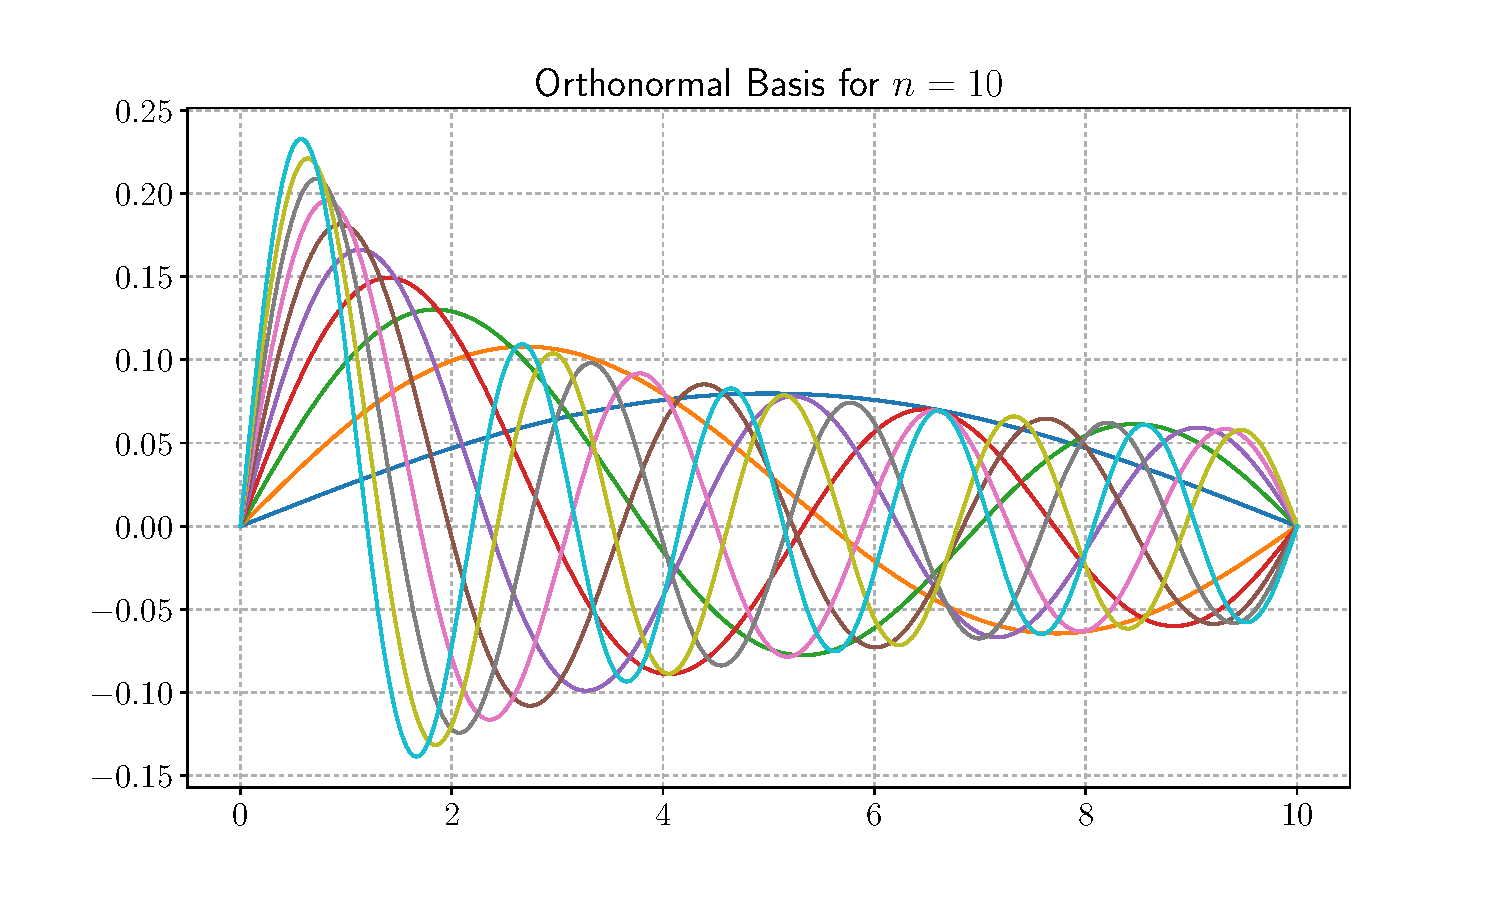
\includegraphics[width=0.95\linewidth]{basis.pdf}
    \caption{10 Orthonormal Basis Functions with \(r_\text{max} = 10\)}\label{fig:basis}
\end{figure}

With the basis at hand we can build the objective function (\ref{eq:objfun}),
that is the function we wish to minimize. To satisfy (\ref{eq:approxcons}) we
begin with the initial guess given by \(\left(\sqrt{\frac{J_0}{n}}, \sqrt{\frac{J_0}{n}}, \ldots, \sqrt{\frac{J_0}{n}}\right)\).
With an objective function, an initial guess, and a constraint, we can use
SciPy's \texttt{scipy.optimize.minimize} to carry out the
minimization\footnote{In order to have this function succeed for large values of
\(n\), that is a large basis set, the maximum number of iterations must be
increased to reach the minimum.}. To reproduce the results in~\cite{spinningq},
in particular, Figure 6, we chose parameters \(a = 2, b = 1.1, \lambda = 1\) and
with \(J_0 = 30\) we obtain the following solution.
\begin{figure}[H]
    \centering
    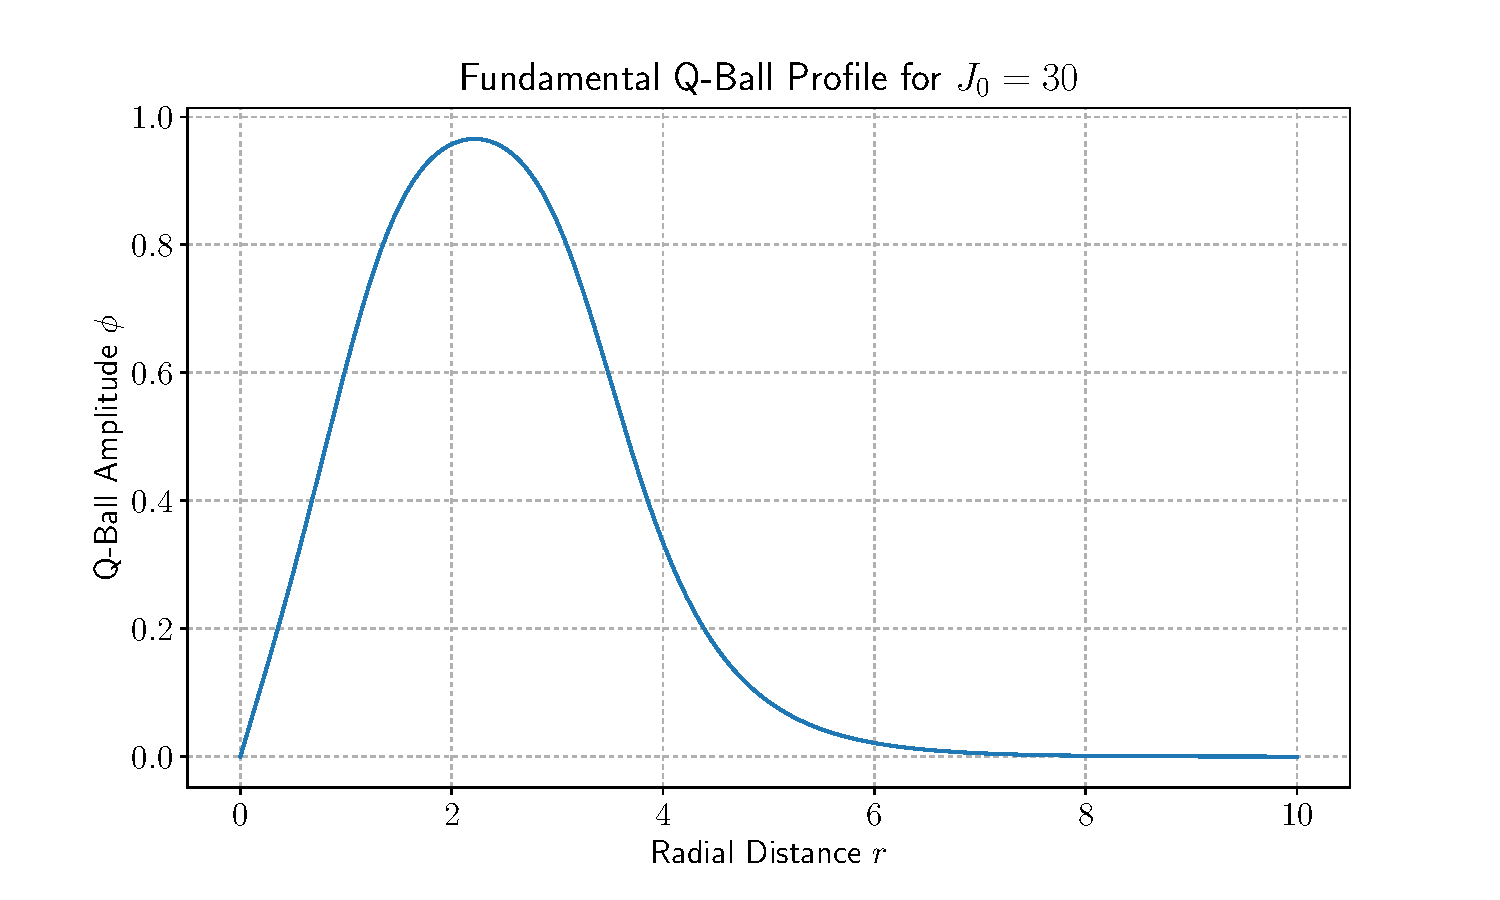
\includegraphics[width=0.95\linewidth]{qballprof30.pdf}
    \caption{\(N = 1\) Excitation of Q-Vortex Solution}\label{fig:profile30}
\end{figure}
This plot was generated with 50 basis functions and an \(x\)-axis sampled 1000
times, i.e. \(\dd{x} = 0.01\). With this solution we can then go on to calculate
the Lagrange multiplier \(\omega^2\) that we saw in Lemma~\ref{lem:nonlineig}.
To calculate \(\omega^2\), we take the \(\delta I\) and \(\delta J\) as defined
in Lemma~\ref{lem:nonlineig}, and take the test function \(\psi\) to be exactly
\(\phi\). This may seem like cheating, however \(\delta I = \chi\delta J\)
should hold for all \(\psi\), and in particular \(\psi = \phi\). We can then
numerically calculate \(\delta I\) and \(\delta J\), calculate the Lagrange
multiplier by taking the quotient \(\chi = \frac{\delta I}{\delta J}\), and then
using the relation \(4\pi\chi = \omega^2\) we have \(\omega = \sqrt{4\pi\chi}\).
For the plot above this yields \(\omega = 0.7216\).

We can then run this procedure for multiple values of \(N\) to further
understand how the Q-Vortex behaves with larger \(N\) values. We note how, as we
increase \(N\), the peak of the soliton moves outward similar to how objects
with more angular momentum tend to increase their radii.
\begin{figure}[H]
    \centering
    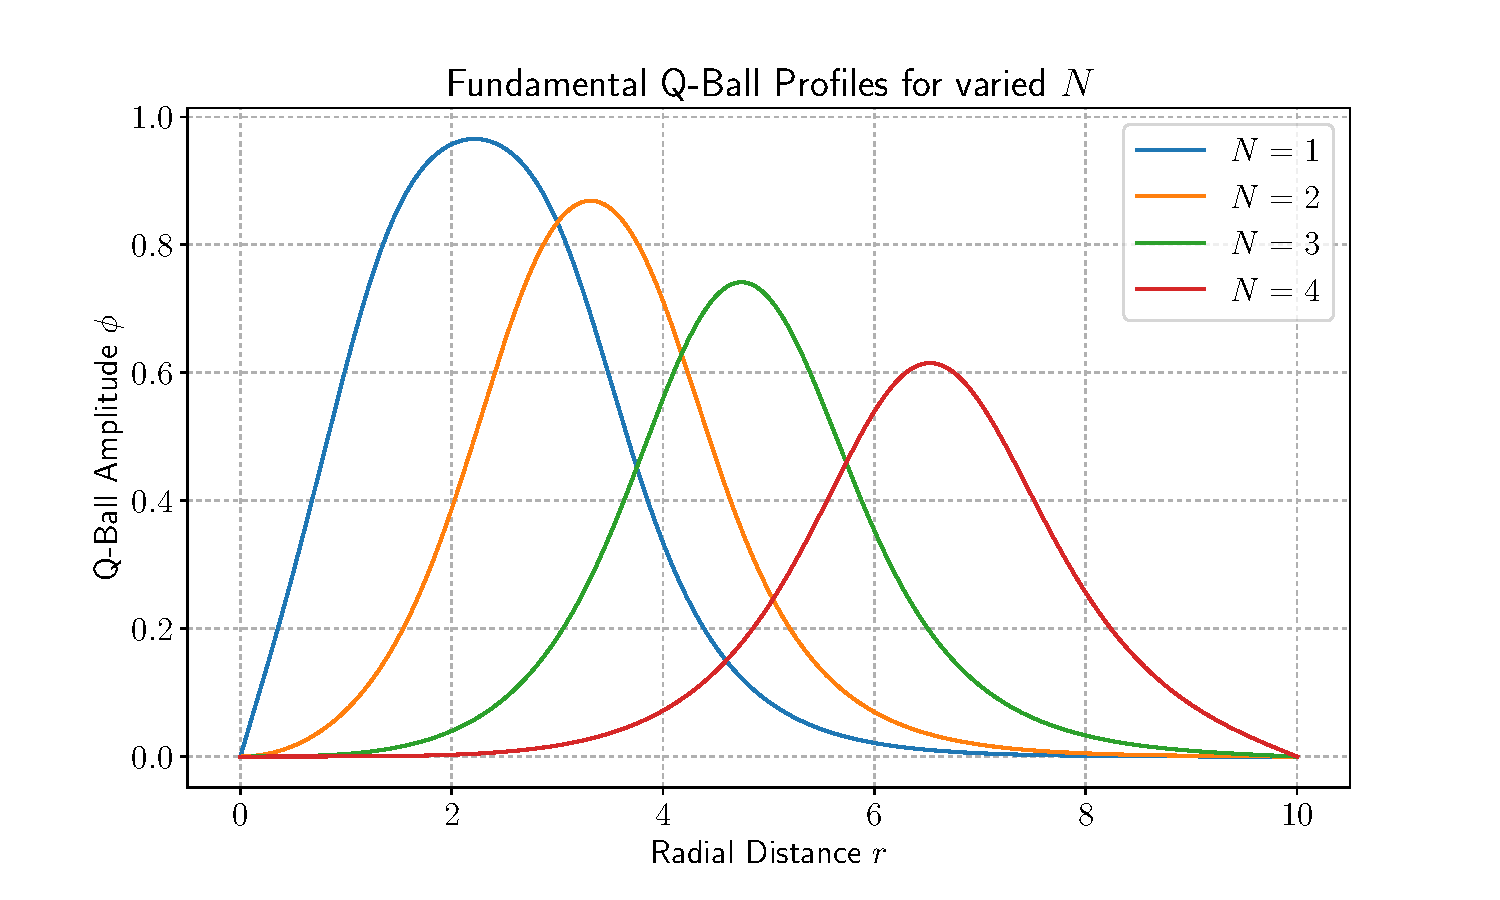
\includegraphics[width=0.95\linewidth]{qballprofs.pdf}
    \caption{First Four Fundamental Q-Vortex Solutions}\label{fig:profiles}
\end{figure}
Now that we have solutions at hand, it is important to understand the error
associated with them. To measure the error we use the following idea and metric.
If the solutions computed above are accurate, they should of course satisfy the
equation of motion (\ref{eq:DE}). Thus we can add everything to one side,
multiply by \(r^2\), square the differential equation, and integrate\footnote{We
multiply by \(r^2\) to make our lives easier so we don't have to deal with the
inverse powers of \(r\) numerically.}.
\begin{equation}
    \mathrm{error} = \int_0^R \left(r\left(r\phi_{r}\right)_r + \omega^2r^2\phi - N^2\phi - \lambda r^2\left(6\phi^5 - 4a\phi^3 + 2b\phi\right)\right)^2\dd{r}
\end{equation}
We can then tabulate the associated values for each solution shown in
Figure~\ref{fig:profiles}.
\begin{table}[H]
    \centering
    \begin{tabular}{c c c}            \toprule
        \(N\) & \(\omega\) & error   \\ \midrule
        1     & 0.72156    & 0.00626 \\ \midrule
        2     & 0.85271    & 0.00084 \\ \midrule
        3     & 1.01243    & 0.00021 \\ \midrule
        4     & 1.16983    & 0.01622 \\ \bottomrule
    \end{tabular}
    \caption{Parameters for \(J_0 = 30\)}\label{tab:params}
\end{table}

It is then natural to ask, for a given \(N\), how does omega change as we vary
the power \(J_0\). Below we see that as the power is increased the soliton peak
flattens and moves outward.
\begin{figure}[H]
    \centering
    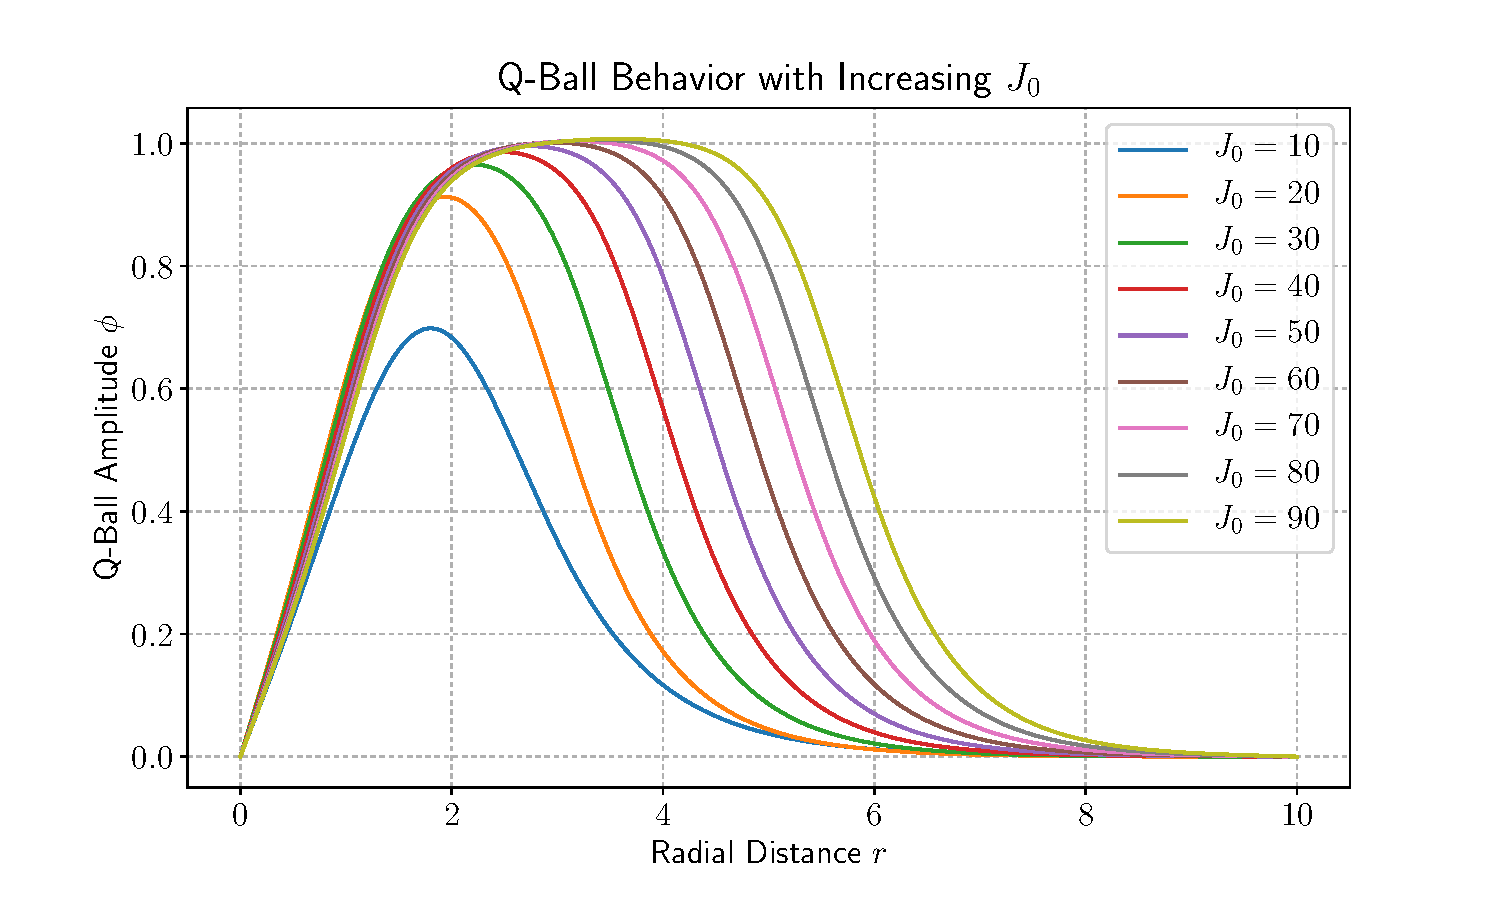
\includegraphics[width=0.95\linewidth]{varypower.pdf}
    \caption{Flat Top Emergence of Q-Vortex Soliton}\label{fig:flattops}
\end{figure}
The parameters for this plot is shown in the table below.
\begin{table}[H]
    \centering
    \begin{tabular}{c c c}              \toprule
        \(J_0\) & \(\omega\) & error   \\ \midrule
        10      & 1.06898    & 0.00002 \\ \midrule
        20      & 0.80058    & 0.00498 \\ \midrule
        30      & 0.72156    & 0.00626 \\ \midrule
        40      & 0.68074    & 0.00137 \\ \midrule
        50      & 0.65481    & 0.00447 \\ \midrule
        60      & 0.63783    & 0.03409 \\ \midrule
        70      & 0.62205    & 0.02264 \\ \midrule
        80      & 0.61019    & 0.00427 \\ \midrule
        90      & 0.60444    & 0.06596 \\ \bottomrule
    \end{tabular}
    \caption{Parameters for \(N = 1\)}\label{tab:paramsN}
\end{table}
It is easy to see in this table that as the power increases, omega not only
decreases, but it looks as though it tends to some number. To investigate this
further we performed a finer scan to understand how the power \(J_0\) effects
\(\omega\).
\begin{figure}[H]
    \centering
    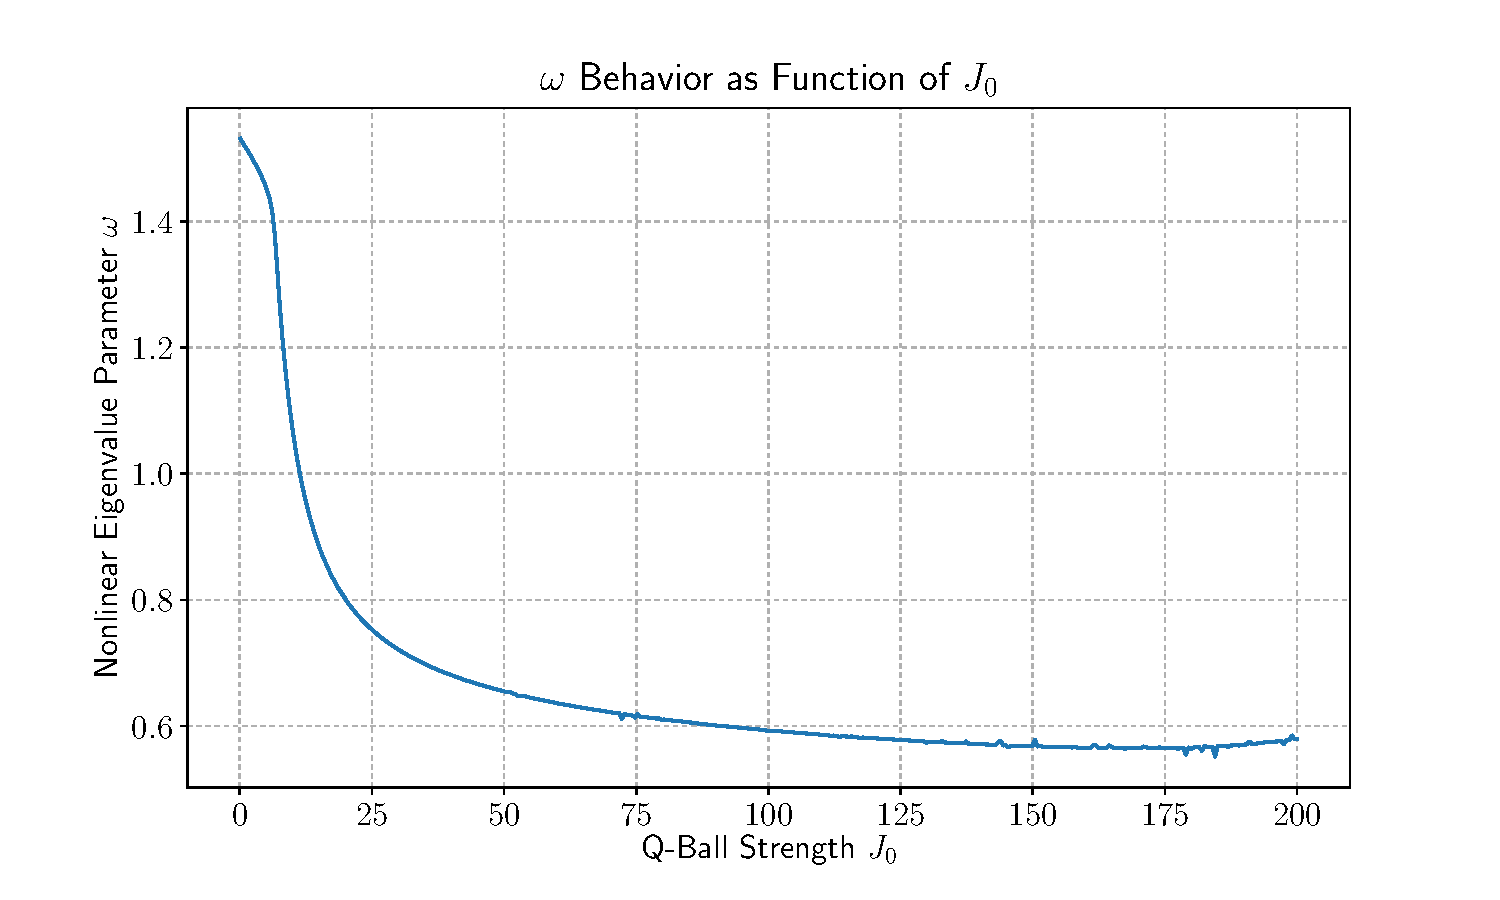
\includegraphics[width=0.95\linewidth]{omegavJ.pdf}
    \caption{\(\omega\) vs. \(J_0\) Parameter Space Scan}\label{fig:paramspace}
\end{figure}
As this plot shows, as we increase the \(J_0\), \(\omega\) falls very quickly at
first, and then more slowly as it dips slightly below 0.6. In particular the
minimum this curve achieves (not including small deviations) is roughly 0.57.







\chapter{Conclusion}\label{chap:conclusion}
\epigraph{Le but de cette thèse est de munir son auteur du titre de Docteur.\\
The goal of this thesis is to furnish its author with the title of Doctor}{Adrien Douady\\\textit{Beginning of A. Douady's thesis}}
Throughout this thesis we have accomplished many things. We began with a
thorough introduction to field theory, assuming only a rudimentary understanding
of classical mechanics. Here we developed ideas that utilized in nearly all
areas of theoretical, and mathematical physics and are paramount for
understanding current research. The highlights were Gauge Theory, the field
theoretic Lagrangian, and of course Noether's Theorem, all of which play an
important role in the work that followed.

To best understand the work that followed, a chapter of the necessary
mathematical prerequisites followed where we introduced fundamental ideas from
functional analysis and the calculus of variations in order to discuss our
problem at hand with a level of rigor.

With the fundamentals from both mathematics, and physics we were able to
introduce Q-Balls. These extremely imporant objects were developped
systematically using the tool from the previous chapters that allowed us to
calculate many important physics quantities such as total energy, angular
momentum, and the stabilizing Noether charge. Once the basic quantities were
calculated, the constrained minimization problem was introduced, and we proved
it was well defined.

The fact that the problem was well defined allowed us to move forward and to
look for solutions numerically. Using a finite element formalism we reduced the
problem to a multivariable calculus minimization problem which is easily solved
numerically. We were then able to compute Q-Ball profiles and their associated
parameters which allow us to understand the objects much better. With the
constrained minimization problem set up we were able to explore parameter space
not previously studied in the literature. In particular we studied how the
Q-Ball changes as one varies the ``strength'' or ``power'' of the object.

While the end of this thesis has come, the work on the problem is certainly not.
There is much more to explore in this field, and in particular this study of
Q-Balls. Further questions are, which potentials have solutions, and are they
qualitatively different from the ones found here? Are the solutions found
unique?\footnote{One way to explore this is to test a variety of points
satisfying the constraint and seeing if they all lead to the same solution.} Can
we decrease the numerical error? There are of course many more interesting
questions to be had, but unfortunately we only had a finite time to answer some.

\appendix
\chapter{Some (possibly) Useful Facts}\label{chap:appendix}
\epigraph{The noblest ambition is that of leaving behind something of permanent
value.}{G.H. Hardy\\\textit{A Mathematicians Apology}}
% chktex-file 21

In this chapter we provide a few ``random'' facts, theorems and arguments that
are not paramount to this thesis, but help it along.

\section{Some Theorems}\label{sec:apptheorems}
\begin{theorem}\label{th:actionexist}
    Let \(X\subseteq\mathbb{R}^n\) be open, and \(\alpha, \beta \in\mathbb{R}_+\)
    with \(\alpha < \beta\). If \(L:[\alpha,\beta]\times X\times \mathbb{R}^n\to\mathbb{R}\)
    is continuously differentiable, then the integral
    \begin{equation}
        S[x(t)]\coloneqq\int_\alpha^\beta L(t, x(t), \dot{x}(t))\dd{t}
    \end{equation}
    exists for all \(x\in\mathrm{C}^1([\alpha,\beta],X)\).
\end{theorem}
This theorem justifies calling \(\mathrm{C}^1(\mathbb{R})\) the domain of the
action as we did in Section~\ref{sec:stationary}. The next theorem is a slightly
more rigorous justification as to when the Euler-Lagrange
equations~\ref{eq:eulerlag} hold.
\begin{theorem}
    If \(x\in\mathrm{C}^1([\alpha,\beta],X)\) is a local extremum of \(S\) as
    defined above, and moreover the function
    \begin{equation}
        [\alpha,\beta]\ni t\mapsto \pdv{\dot{x}}L(t, x(t),\dot{x}(t))
    \end{equation}
    is continuously differentiable, then the following equation holds.
    \begin{equation}
        \pdv{x}L(t, x(t),\dot{x}(t)) = \dv{t}\pdv{\dot{x}}L(t, x(t),\dot{x}(t))
    \end{equation}
\end{theorem}

\begin{theorem}[Poincar\'{e} Inequality]
    Let \(p\in[1,\infty)\) and \(\Omega\) a bounded subset of \(\mathbb{R}\). % chktex 9
    Then there exists a constant \(C\), dependent on \(\Omega\) and \(p\), so
    that for every function \(u\in W^{1,2}(\Omega)\) we have the following
    inequality.
    \begin{equation}
        \|u\|_{L^p(\Omega)} \leq C\|u'\|_{L^p(\Omega)}
    \end{equation}
\end{theorem}


\section{Some Arguments}\label{sec:appargs}
In this section we recreate, with more detail, the original arguments for the
existence of Q-Balls as proposed in~\cite{coleman}.

As Q-Balls were proposed in~\cite{coleman} these objects are described by a
field \(\phi\) that is some constant value inside a volume \(B\), and 0 outside.
There exact energy is given by (\ref{eq:nospinenergy}), and in this
approximation reduces to
\begin{equation}\label{eq:Eapprox}
    E = \frac{1}{2}\omega^2\phi^2B + VB
\end{equation}
and similarly for the Noether Charge (\ref{eq:nospincharge}) we have the following.
\begin{equation}\label{eq:Qapprox}
    Q = \omega \phi^2 B
\end{equation}
The fundamental idea of a Q-Ball is that it's energy configuration is lower than
that of the separate particles, and hence we should minimize the energy for a
given value of the charge \(Q\). In order to do this we eliminate \(\omega\) by
inserting (\ref{eq:Qapprox}) into (\ref{eq:Eapprox}) to obtain
\begin{equation}
    E = \frac{1}{2}\frac{Q^2}{\phi^2 B} + VB.
\end{equation}
Now we minimize this with respect to the volume \(B\) to find it is minimized when
\begin{equation}
    B = \frac{Q}{\sqrt{2\phi^2 V}}.
\end{equation}
With this volume the energy then reads
\begin{align}
    E & = \frac{1}{2}\frac{Q^2}{\phi^2}\frac{\sqrt{2\phi^2 V}}{Q} + \frac{VQ}{\sqrt{2\phi^2 V}} \\
      & = Q\sqrt{2\phi^2 V}\left( \frac{1}{2\phi^2} + \frac{V}{2\phi^2 V}\right) \\
      & = Q \sqrt{\frac{2V}{\phi^2}}.
\end{align}
The last step is then to minimize this value with respect to \(\phi\) in order
to obtain
\begin{equation}
    E = \min_\phi Q \sqrt{\frac{2V}{\phi^2}}
\end{equation}
which is where the restriction on \(\omega\) comes from as seen in
(\ref{eq:omegabounds}). The upper bound for \(\omega\) arises from considering
the qualitative shape of the potential, and a more detailed description of its
derivation can be found in~\cite{coleman, qball6}.

This construction of Q-Balls allows the energy configuration of the ``Q-matter''
as Coleman calls it to be lower than that of the separate particles floating
around in space.

\bibliographystyle{unsrt}
\bibliography{refs}

\end{document}
